\documentclass[11pt, a4paper]{article}

% --- Typography ---
\usepackage[T1]{fontenc}
\usepackage[utf8]{inputenc}
\usepackage{tgpagella}
\usepackage[scaled=0.85]{beramono}
\usepackage{microtype}

% --- Layout ---
\usepackage[
  top=1.25in,
  bottom=1.25in,
  left=1.25in,
  right=1.25in
]{geometry}
\usepackage{setspace}
\setstretch{1.4}

% --- Headers & Sections ---
\usepackage{fancyhdr}
\usepackage{titlesec}
\usepackage{xcolor}

\definecolor{darkblue}{RGB}{0, 51, 102}
\definecolor{codebg}{RGB}{245, 245, 245}
\definecolor{codeframe}{RGB}{200, 200, 200}

\titleformat{\section}
  {\Large\bfseries\color{darkblue}}
  {\thesection.}{0.5em}{}
\titleformat{\subsection}
  {\large\bfseries\color{darkblue}}
  {\thesubsection}{0.5em}{}
\titleformat{\subsubsection}
  {\normalsize\bfseries}
  {\thesubsubsection}{0.5em}{}

\pagestyle{fancy}
\fancyhf{}
\fancyhead[L]{\small\textit{How to Build AI Agents}}
\fancyhead[R]{\small\textit{\nouppercase{\leftmark}}}
\fancyfoot[C]{\thepage}
\renewcommand{\headrulewidth}{0.4pt}

% --- Code listings ---
\usepackage{listings}
\lstset{
  backgroundcolor=\color{codebg},
  frame=single,
  rulecolor=\color{codeframe},
  basicstyle=\ttfamily\small,
  keywordstyle=\color{darkblue}\bfseries,
  commentstyle=\color{gray}\itshape,
  stringstyle=\color{teal},
  breaklines=true,
  breakatwhitespace=true,
  tabsize=4,
  showstringspaces=false,
  aboveskip=1em,
  belowskip=1em,
  xleftmargin=1em,
  xrightmargin=1em,
  numbers=none,
}

% --- Tables ---
\usepackage{booktabs}
\usepackage{longtable}
\usepackage{array}

% --- Graphics ---
\usepackage{graphicx}
\graphicspath{{./}}

% --- Links ---
\usepackage[
  colorlinks=true,
  linkcolor=darkblue,
  urlcolor=darkblue,
  citecolor=darkblue
]{hyperref}

% --- Lists ---
\usepackage{enumitem}
\setlist{nosep, leftmargin=1.5em}

% Pandoc requirements
\providecommand{\tightlist}{%
  \setlength{\itemsep}{0pt}\setlength{\parskip}{0pt}}
\newcommand{\passthrough}[1]{#1}

% CSL refs support

\begin{document}

% --- Custom title page ---
\begin{titlepage}
\vspace*{3cm}
\begin{center}
{\Huge\bfseries\color{darkblue} How to Build AI Agents}\\[0.8em]
{\Large A Practitioner's Manual}\\[2em]
{\large Version 1.0 \quad\textperiodcentered\quad March 2026}\\[3em]
{\normalsize\textit{Produced by Yggdra Research System}}\\[1em]
{\small Intended audience: Software engineers, technical leads, and\\
technology decision-makers evaluating or building AI agent systems.\\
No prior experience with AI agents is assumed;\\
familiarity with programming concepts is helpful but not required.}
\end{center}
\vfill
\end{titlepage}

\hypertarget{abstract}{%
\subsection{Abstract}\label{abstract}}

AI agents --- software systems where a large language model dynamically
decides what actions to take rather than following a predetermined
script --- have become one of the most discussed topics in software
engineering. The promise is compelling: autonomous systems that can
research, code, analyze, and coordinate complex tasks with minimal human
oversight. The reality, as of early 2026, is more nuanced. Ninety-five
percent of enterprise AI pilots fail to reach production. Multi-agent
systems see 40\% pilot failure rates within six months. A single runaway
agent generated a \$47,000 API bill over eleven days before anyone
noticed.

This manual is a practitioner's guide to building AI agents that
actually work. It synthesizes findings from over fifty research papers,
fourteen original research reports, six production codebases, and three
years of collective deployment experience. The document covers the full
lifecycle: from deciding whether you need an agent at all, through
architecture selection, context management, multi-agent coordination,
evaluation, and production deployment. Each chapter builds on a single
running example --- a literature research agent that starts as a
twenty-line script and evolves, chapter by chapter, into a
production-grade system with evaluation, memory, and human oversight.

The manual's central argument is that the scaffolding around the model
--- the tools, the context management, the evaluation infrastructure,
the safety controls --- provides roughly eighty percent of the value in
any agent system. The model itself provides twenty percent. Most
failures come not from model limitations but from architectural
decisions: too many tools, too little evaluation, no cost controls, and
insufficient human oversight at critical decision points.

\begin{center}\rule{0.5\linewidth}{0.5pt}\end{center}

\hypertarget{introduction}{%
\subsection{1. Introduction}\label{introduction}}

Imagine you ask an AI system to research a topic and write a summary. In
a traditional setup, you would write a prompt, send it to a language
model, and receive a response. The system does one thing: it generates
text based on your input. If the response is incomplete or wrong, you
refine your prompt and try again. The human drives the process.

Now imagine a different system. You give it the same research task, but
instead of generating a single response, it begins to \emph{act}. It
searches the web for relevant papers. It reads them. It decides that
three of the five papers are not relevant and discards them. It notices
a gap in its understanding and searches again with different terms. It
drafts a summary, reviews its own draft, identifies a factual error,
goes back to the source to verify, corrects the error, and presents the
final result. The system drove the process. You provided the goal; it
decided the steps.

The first system is a language model. The second is an agent.

This distinction --- between systems where humans decide the control
flow and systems where the model decides --- is the foundation of
everything in this manual. It is also the source of most confusion in
the field, because the industry uses the word ``agent'' to describe
everything from a chatbot with a search tool to a fully autonomous
system that operates for hours without human input. This manual will be
precise about what these terms mean, because precision prevents the kind
of architectural mistakes that lead to failed deployments and unexpected
bills.

\hypertarget{why-this-manual-exists}{%
\subsubsection{Why This Manual Exists}\label{why-this-manual-exists}}

The current landscape of AI agent development is caught between two
extremes. On one side, marketing materials promise autonomous AI
employees that will transform every business process. On the other,
practitioners who have actually deployed agents report sobering failure
rates: seventy-five percent of agentic AI tasks fail in production when
measured on real workflows (Superface, 2025), and only eleven percent of
organizations have agentic AI running in production as of late 2025
(Cleanlab, 2025).

Between the hype and the disillusionment lies a productive middle
ground. Certain agent architectures genuinely work --- coding
assistants, customer support deflection, structured research --- when
they are built with appropriate expectations, proper evaluation, and
honest assessment of what the technology can and cannot do. This manual
maps that middle ground.

\hypertarget{what-this-manual-covers}{%
\subsubsection{What This Manual Covers}\label{what-this-manual-covers}}

The document is organized into eight chapters that follow the lifecycle
of building an agent system:

\textbf{Chapter 2} establishes the foundations: what agents actually
are, the spectrum of automation from cron jobs to autonomous systems,
and a framework for deciding whether you need an agent at all. It
introduces the compounding reliability problem --- the mathematical fact
that explains why most agent demos work and most agent deployments do
not.

\textbf{Chapter 3} catalogs the architecture patterns available to agent
builders, from simple prompt chains through the ReAct loop\footnote{\textbf{ReAct}
  stands for ``Reason + Act,'' an architecture where the model
  alternates between thinking about what to do and taking an action. It
  was introduced by Yao et al.~(2023) and is the default pattern in most
  agent frameworks.} to plan-and-execute architectures. It examines the
minimalist philosophy articulated by practitioners like Mario Zechner
and Armin Ronacher, who argue that four tools are sufficient for most
agent tasks.

\textbf{Chapter 4} addresses context engineering --- the discipline of
managing what information the model sees at each step. This is arguably
the most important chapter, because context management is where most
agent failures originate and where most performance gains are found.

\textbf{Chapter 5} covers multi-agent systems: when you need more than
one agent, how they communicate, and a detailed examination of the major
frameworks (LangGraph, CrewAI, AutoGen, and others). It includes honest
cost analysis and guidance on when multi-agent coordination helps versus
when it makes things worse.

\textbf{Chapter 6} tackles evaluation and observability --- how to know
whether your agent is working correctly when its behavior is
non-deterministic and its outputs cannot be verified with simple
assertions.

\textbf{Chapter 7} addresses production concerns: failure rates, safety
controls, cost management, and the human-in-the-loop patterns that make
agents viable in real deployments.

\textbf{Chapter 8} provides implementation guidance with runnable code
examples that build on the concepts from earlier chapters.

\hypertarget{the-running-example}{%
\subsubsection{The Running Example}\label{the-running-example}}

Throughout this manual, we follow the construction of a single system: a
\textbf{literature research agent}. In Chapter 2, it begins as a simple
Python script that searches for papers and prints their titles. By
Chapter 3, it gains the ability to read papers and decide which ones are
relevant. In Chapter 4, it learns to manage its own context as the
number of papers grows. By Chapter 5, it coordinates multiple
specialized sub-agents. In Chapter 6, it acquires evaluation
infrastructure. By Chapter 7, it runs in production with cost controls
and human oversight.

This is not a hypothetical example. The architecture mirrors real
systems that the authors have built and operated, including the research
system that produced this manual.

\begin{center}\rule{0.5\linewidth}{0.5pt}\end{center}

\hypertarget{foundations-what-agents-are-and-when-you-need-one}{%
\subsection{2. Foundations: What Agents Are and When You Need
One}\label{foundations-what-agents-are-and-when-you-need-one}}

\hypertarget{the-line-between-workflows-and-agents}{%
\subsubsection{2.1 The Line Between Workflows and
Agents}\label{the-line-between-workflows-and-agents}}

The most useful definition of an AI agent comes from Anthropic's
engineering team, who drew a clean distinction in their influential
guide ``Building Effective Agents'' (Anthropic, 2024):

\begin{quote}
\textbf{Workflows} are systems where LLMs are orchestrated through
predefined code paths. The developer decides the control flow at design
time.

\textbf{Agents} are systems where LLMs dynamically direct their own
processes and tool usage. The model decides the control flow at runtime.
\end{quote}

This distinction matters because the engineering requirements are
fundamentally different. A workflow can be tested with conventional
software testing: given these inputs, does step three produce the
expected output? An agent cannot, because the sequence of steps is not
predetermined. The model might call two tools or twelve. It might
succeed on the first attempt or enter a retry loop. Testing an agent
requires evaluating \emph{trajectories} --- sequences of decisions ---
not just final outputs.

Here is a practical test to determine which category your system falls
into: \textbf{Can you draw the complete control flow on a whiteboard
before the system runs?} If you can enumerate every possible path
through the system, you are building a workflow. If the model must
decide at runtime which path to take based on intermediate results, you
are building an agent. Most systems that are marketed as agents are, by
this definition, workflows --- and that is perfectly fine. Workflows are
more reliable, cheaper to operate, and easier to debug.

\hypertarget{the-automation-spectrum}{%
\subsubsection{2.2 The Automation
Spectrum}\label{the-automation-spectrum}}

Before reaching for an agent, it is worth understanding the full
spectrum of automation options. Each level adds capability but also adds
complexity, cost, and failure modes. The right choice is the simplest
level that solves the problem.

\begin{figure}
\centering
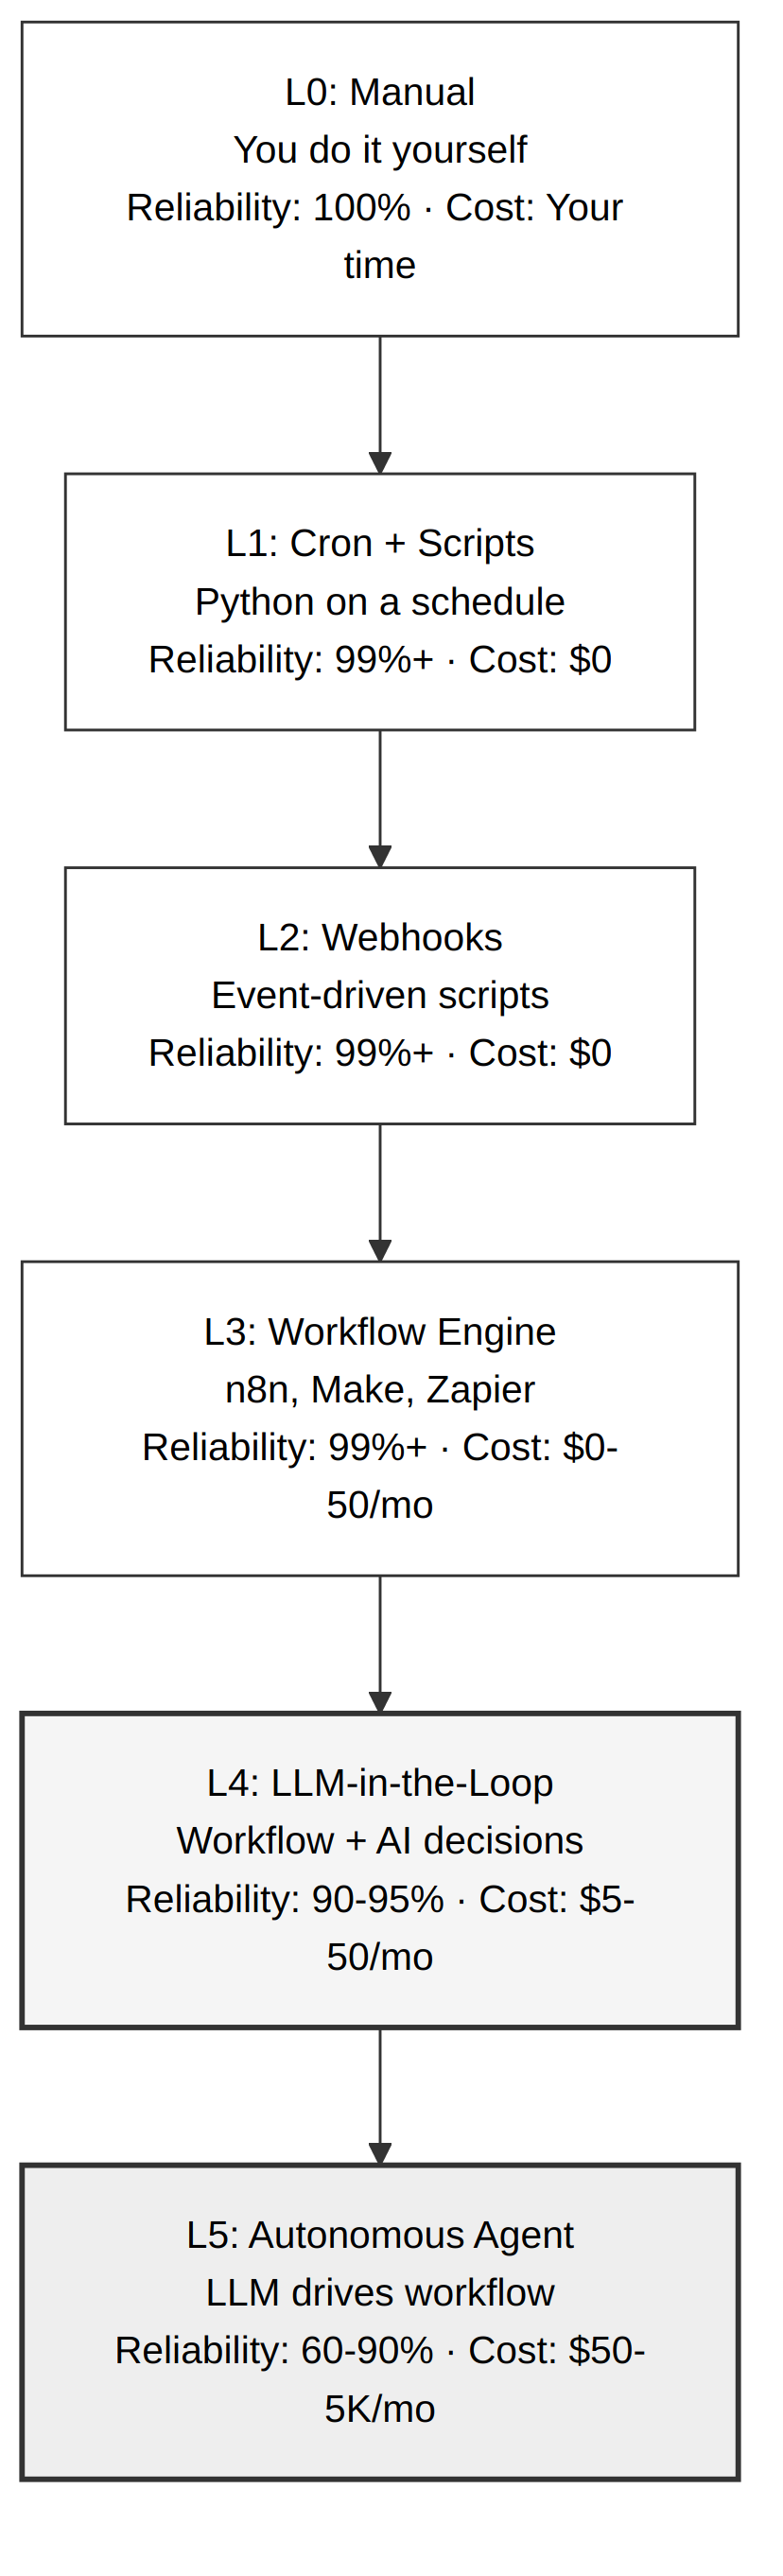
\includegraphics[width=0.85\textwidth,height=\textheight]{figures/diagram_1.png}
\caption{Figure 1. The automation spectrum. Green levels (L0--L3) are
deterministic and highly reliable. Amber (L4) introduces AI at specific
decision points. Red (L5) gives the AI control over the entire workflow.
Most automation problems are L1--L3 problems}
\end{figure}

\textbf{Level 0: Manual.} You do the task yourself. This is where every
process starts, and where most processes should remain until they occur
more than twice per week. The advantage is perfect reliability --- you
understand the task, and you can handle exceptions. The disadvantage is
that your time is the bottleneck.

\textbf{Level 1: Cron jobs and scripts.} A Python script runs on a
schedule. It fetches data, transforms it, writes results to a file or
database. No user interface, no framework, no dependencies beyond the
standard library. It runs at four in the morning, does its job, and
nobody thinks about it until something breaks --- which is the highest
compliment you can give to a piece of infrastructure. The research
system that produced this manual runs eight cron jobs. In six weeks of
continuous operation, the total number of failures has been zero.

\textbf{Level 2: Webhooks and event-driven scripts.} Something happens
in the external world --- a message arrives, a file is uploaded, a
database record changes --- and a script responds. The trigger is
external rather than time-based, but the processing is still
deterministic. Still simple. Still reliable.

\textbf{Level 3: Workflow engines.} Tools like n8n, Make, or Zapier
connect multiple services through visual pipelines. When you need to
pull data from one API, transform it, check a condition, and push the
result to another API, a workflow engine handles the plumbing. The logic
is predefined; the engine handles retries, error notifications, and
scheduling.

\textbf{Level 4: LLM-in-the-loop.} This is the hybrid pattern\footnote{The
  \textbf{hybrid pattern} combines deterministic workflow steps with one
  or more LLM decision nodes. The workflow handles data flow, error
  handling, and retries; the LLM handles the single step that requires
  natural language understanding or judgment.} that deserves far more
attention than it receives. The workflow is still deterministic --- data
flows through predefined steps --- but at one specific point, an LLM
makes a judgment call. It might classify an incoming email into
categories, extract structured data from an unstructured document, or
decide which of three response templates best fits a customer inquiry.
The key characteristic is that the LLM is a \emph{function call within a
pipeline}, not the orchestrator of the pipeline.

A 2025 arxiv paper titled ``Blueprint First, Model Second'' describes
this approach: the LLM is ``strategically reframed as no longer the
central decision-maker but is invoked as a specialized tool at specific
nodes.'' This is arguably the most cost-effective way to use large
language models in production, because it combines the reliability of
deterministic workflows with the flexibility of AI at the single point
where flexibility is needed.

\textbf{Level 5: Autonomous agents.} The LLM drives the entire workflow.
It decides which tools to call, in what order, with what parameters. It
evaluates the results of each step and decides what to do next. This is
the level that generates the most excitement --- and the most failures.

The critical insight is that \textbf{most automation problems are Level
1 through 3 problems}. The industry hype concentrates on Level 5, but a
cron job has never been cancelled for ``unclear business value.'' Before
building an agent, work through the spectrum from the bottom up and stop
at the first level that solves your problem.

\hypertarget{our-running-example-at-level-1}{%
\paragraph{Our Running Example at Level
1}\label{our-running-example-at-level-1}}

To illustrate the spectrum concretely, consider the literature research
task introduced in Chapter 1. At Level 1, the simplest version is a cron
job:

\begin{lstlisting}[language=Python]
# research_cron.py -- runs daily at 08:00
import requests

ARXIV_API = "http://export.arxiv.org/api/query"

def search_papers(query: str, max_results: int = 5) -> list[dict]:
    """Search arXiv for recent papers matching a query."""
    response = requests.get(ARXIV_API, params={
        "search_query": f"all:{query}",
        "sortBy": "submittedDate",
        "sortOrder": "descending",
        "max_results": max_results
    })
    # Parse XML response, extract titles and abstracts
    papers = parse_arxiv_xml(response.text)
    return papers

if __name__ == "__main__":
    papers = search_papers("AI agent evaluation")
    for paper in papers:
        print(f"- {paper['title']} ({paper['date']})")
\end{lstlisting}

This script is twenty lines of code. It runs reliably. It does exactly
one thing: search arXiv and list results. It does not decide what to
search for (the query is hardcoded), it does not read the papers, and it
does not judge which ones are relevant. Those are human tasks. For many
research needs, this is sufficient --- and it costs nothing to operate.

The question this manual answers is: when is this not enough, and what
do you build instead?

\hypertarget{the-compounding-reliability-problem}{%
\subsubsection{2.3 The Compounding Reliability
Problem}\label{the-compounding-reliability-problem}}

The single most important fact about AI agents is a mathematical one,
and understanding it will save you from the most common category of
deployment failure.

Consider an agent that completes a task in five steps, where each step
succeeds with ninety-five percent probability. The probability that all
five steps succeed is not ninety-five percent --- it is 0.95 raised to
the fifth power, which equals seventy-seven percent. For a ten-step
agent, the success rate drops to sixty percent. For twenty steps, it
falls to thirty-six percent.

\begin{figure}
\centering
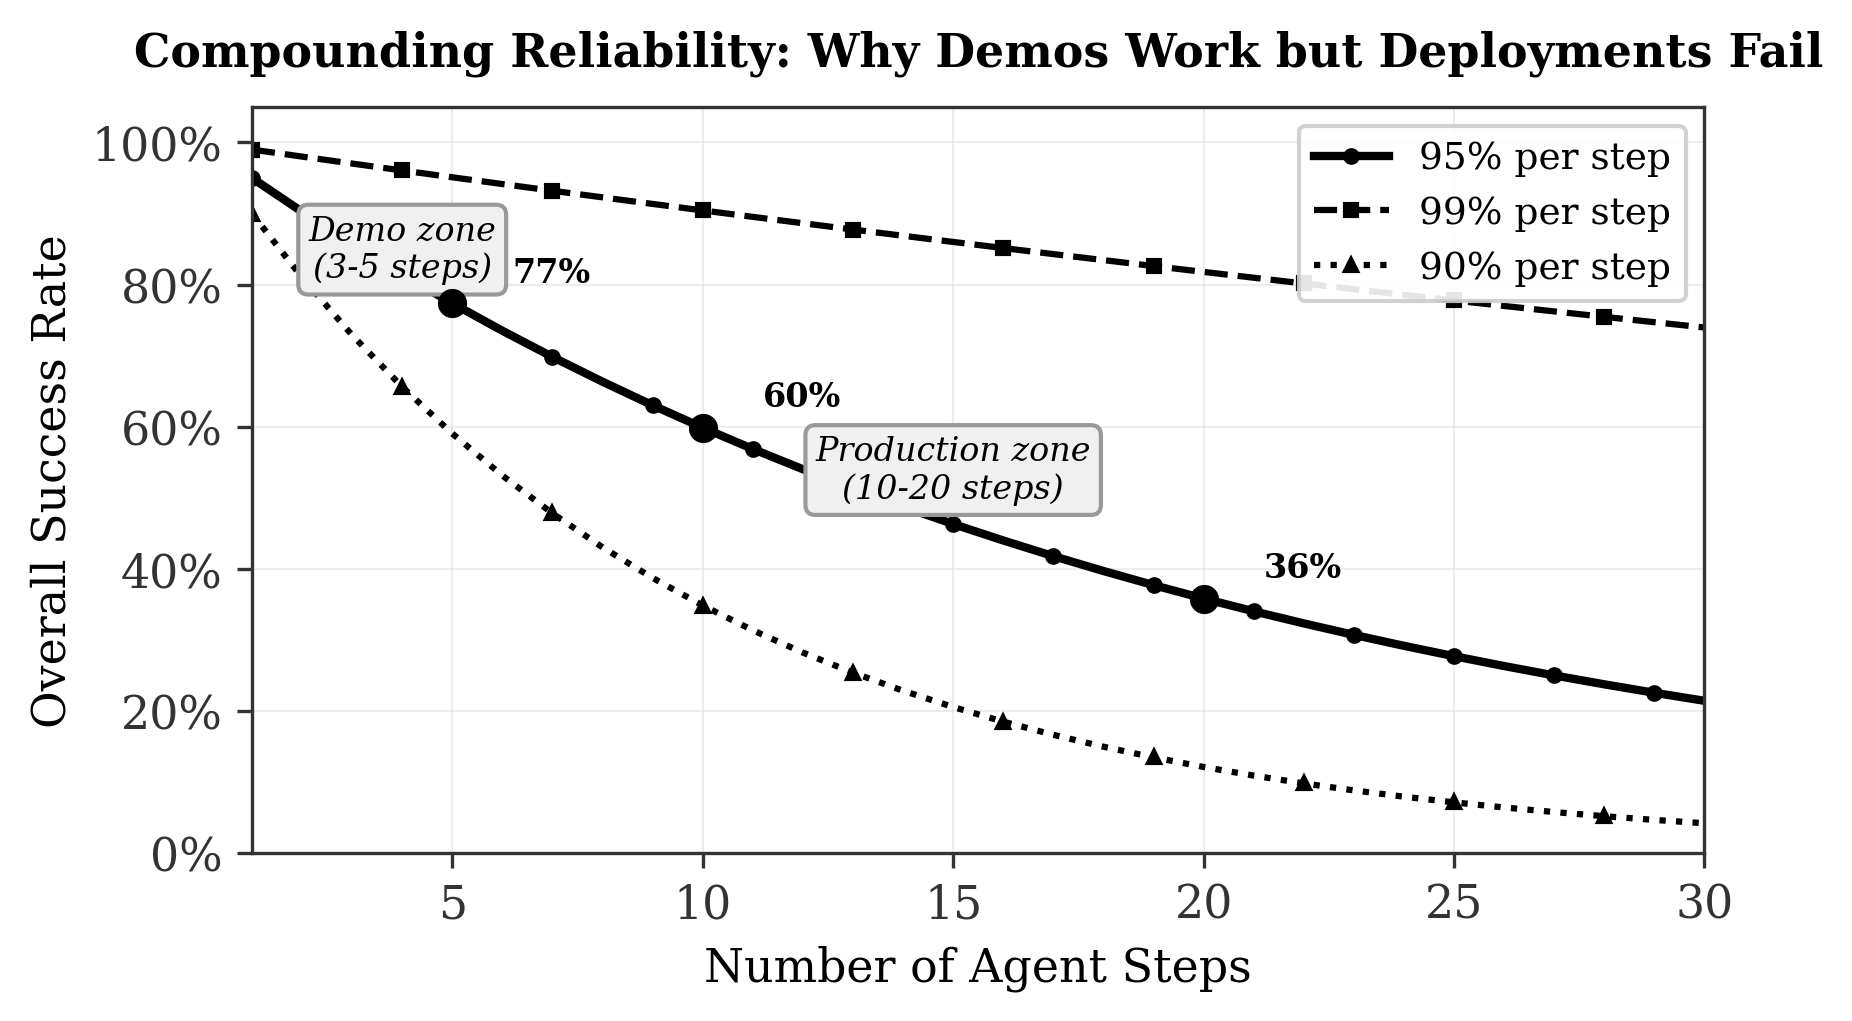
\includegraphics[width=0.85\textwidth,height=\textheight]{figures/diagram_2.png}
\caption{Figure 2. The compounding reliability problem. Even with 95\%
per-step reliability, agent success rates decline exponentially with the
number of steps. A twenty-step agent succeeds only 36\% of the time}
\end{figure}

This exponential decay is the \textbf{compounding reliability problem},
and it explains nearly every observation about AI agents in production:

It explains why \textbf{demos work but deployments fail}. A demo with
three carefully chosen steps succeeds eighty-six percent of the time ---
impressive enough to secure funding. A production deployment with
fifteen steps succeeds only forty-six percent of the time ---
frustrating enough to get cancelled.

It explains why \textbf{ninety-five percent of enterprise AI pilots
fail} to reach production (Zhang, 2025). The pilots work in controlled
conditions with simple tasks. Scaling to real complexity multiplies the
number of steps, and the compounding effect destroys reliability.

It explains why \textbf{Gartner predicts that forty percent of agentic
AI projects will be scrapped by 2027}. Organizations discover the
compounding problem through painful experience rather than through
analysis before deployment.

And it explains the most important architectural principle in this
manual: \textbf{the fix is not better models --- it is fewer steps,
human checkpoints at critical points, and honest assessment of whether
you need an agent at all.} A twenty-step agent with ninety-five percent
per-step reliability and a human checkpoint at step ten has an overall
success rate of sixty percent for the first half and sixty percent for
the second half, with the human correcting errors at the midpoint. The
effective success rate is dramatically higher than the thirty-six
percent of the unchecked version, because errors caught at the
checkpoint do not cascade into subsequent steps.

\hypertarget{the-state-of-the-field-march-2026}{%
\subsubsection{2.4 The State of the Field (March
2026)}\label{the-state-of-the-field-march-2026}}

Before building an agent, it is worth understanding the current
empirical landscape --- not the marketing landscape, but the measured
one.

\textbf{What works well.} Coding agents with human oversight are the
strongest category. Tools like Claude Code, Cursor, and GitHub Copilot
deliver genuine productivity gains on well-defined, bounded tasks.
Claude Opus 4.5 leads the SWE-bench Verified benchmark at 80.9\% on
resolving real GitHub issues end-to-end (SWE-bench, 2026). Customer
support agents that handle routine inquiries (tier-1 deflection) are the
most production-proven category, achieving fifty to sixty-five percent
automated resolution of incoming queries (Salesforce, 2025). Research
and analysis agents --- systems that gather, organize, and summarize
information from multiple sources --- are effective when the task has
clear parameters and the user reviews the output.

\textbf{What does not work yet.} Fully autonomous business processes
remain largely aspirational: only eleven percent of organizations have
agentic AI in production (Cleanlab, 2025). Multi-agent systems at scale
fail forty percent of the time within six months, with coordination
overhead often destroying any theoretical benefits (Gartner, 2025).
Computer use agents --- systems that interact with graphical interfaces
--- produce impressive demonstrations but are too fragile for production
workflows because GUI layouts change unpredictably.

\textbf{The METR bombshell.} Perhaps the most sobering data point comes
from METR (Model Evaluation \& Threat Research), who conducted a
randomized controlled trial with sixteen experienced open-source
developers on 246 real coding issues. Their finding: developers using AI
tools were \textbf{nineteen percent slower} than developers working
without AI tools. The developers \emph{perceived} themselves as faster
--- they reported feeling twenty to thirty percent more productive ---
but objective screen recordings told the opposite story (METR, 2025).
This finding has direct implications for agent evaluation: self-reported
effectiveness is unreliable. You need instrumented, automated
measurement.

\hypertarget{deciding-whether-to-build-an-agent}{%
\subsubsection{2.5 Deciding Whether to Build an
Agent}\label{deciding-whether-to-build-an-agent}}

Given the compounding reliability problem and the current state of the
field, the decision to build an agent should not be taken lightly. Here
is a structured framework for making that decision:

\textbf{Question 1: Can you enumerate the possible execution paths?} If
you can list every possible sequence of steps the system might take, you
do not need an agent. Build a workflow. Workflows are deterministic,
testable, and cheap. Most problems have enumerable paths once you think
carefully about them.

\textbf{Question 2: Does exactly one step require natural language
judgment?} If the rest of the process is well-defined but one step needs
the model to classify, extract, or decide, use the hybrid pattern (Level
4). Insert the LLM as a function call at that single decision point and
keep everything else deterministic.

\textbf{Question 3: Is the input space genuinely unpredictable?} Only if
the possible inputs are so varied that you cannot write rules to handle
them should you consider a true agent. Even then, start with a single
agent with a small number of well-designed tools.

\textbf{Question 4: Is the blast radius bounded?} An agent that can only
read and write files in a single directory is fundamentally safer than
one with unrestricted system access. Bound the agent's capabilities to
the minimum necessary for the task.

\textbf{Question 5: Can you define and measure success?} If you cannot
specify what a correct outcome looks like, you cannot evaluate the
agent, which means you cannot know whether it is working. Define success
criteria before writing a single line of code.

\textbf{Question 6: Is the cost of failure acceptable?} Apply the
two-way door principle\footnote{The \textbf{two-way door principle},
  borrowed from Amazon's decision-making framework, distinguishes
  between reversible decisions (two-way doors, where you can walk back
  through if the outcome is wrong) and irreversible decisions (one-way
  doors, where the consequences are permanent). For agents, reversible
  actions can be automated; irreversible actions should require human
  approval.}: if the agent's actions are reversible (creating a draft
document, generating a code suggestion), let it operate autonomously. If
the actions are irreversible (sending an email to a client, deploying to
production, spending money), require human approval.

If you answer ``no'' to questions three through six, do not build an
agent. Build a workflow, write a script, or keep the process manual. The
most expensive mistake in agent development is building an agent for a
problem that did not need one.

\begin{center}\rule{0.5\linewidth}{0.5pt}\end{center}

\hypertarget{architecture-patterns-how-to-structure-an-agent}{%
\subsection{3. Architecture Patterns: How to Structure an
Agent}\label{architecture-patterns-how-to-structure-an-agent}}

Once you have determined that your problem genuinely requires an agent,
the next decision is how to structure it. This chapter catalogs the
major architecture patterns, starting with the simplest and progressing
to the most complex. The governing principle is: \textbf{use the
simplest pattern that solves the problem.} Complexity is not free ---
every additional layer adds failure modes, debugging difficulty, and
operational cost.

\hypertarget{the-six-composable-patterns}{%
\subsubsection{3.1 The Six Composable
Patterns}\label{the-six-composable-patterns}}

Anthropic's ``Building Effective Agents'' guide (Anthropic, 2024)
identifies six composable patterns that can be combined to build agent
systems. They are listed here in order of increasing complexity, and the
recommendation is to exhaust the simpler options before reaching for the
more complex ones.

\begin{figure}
\centering
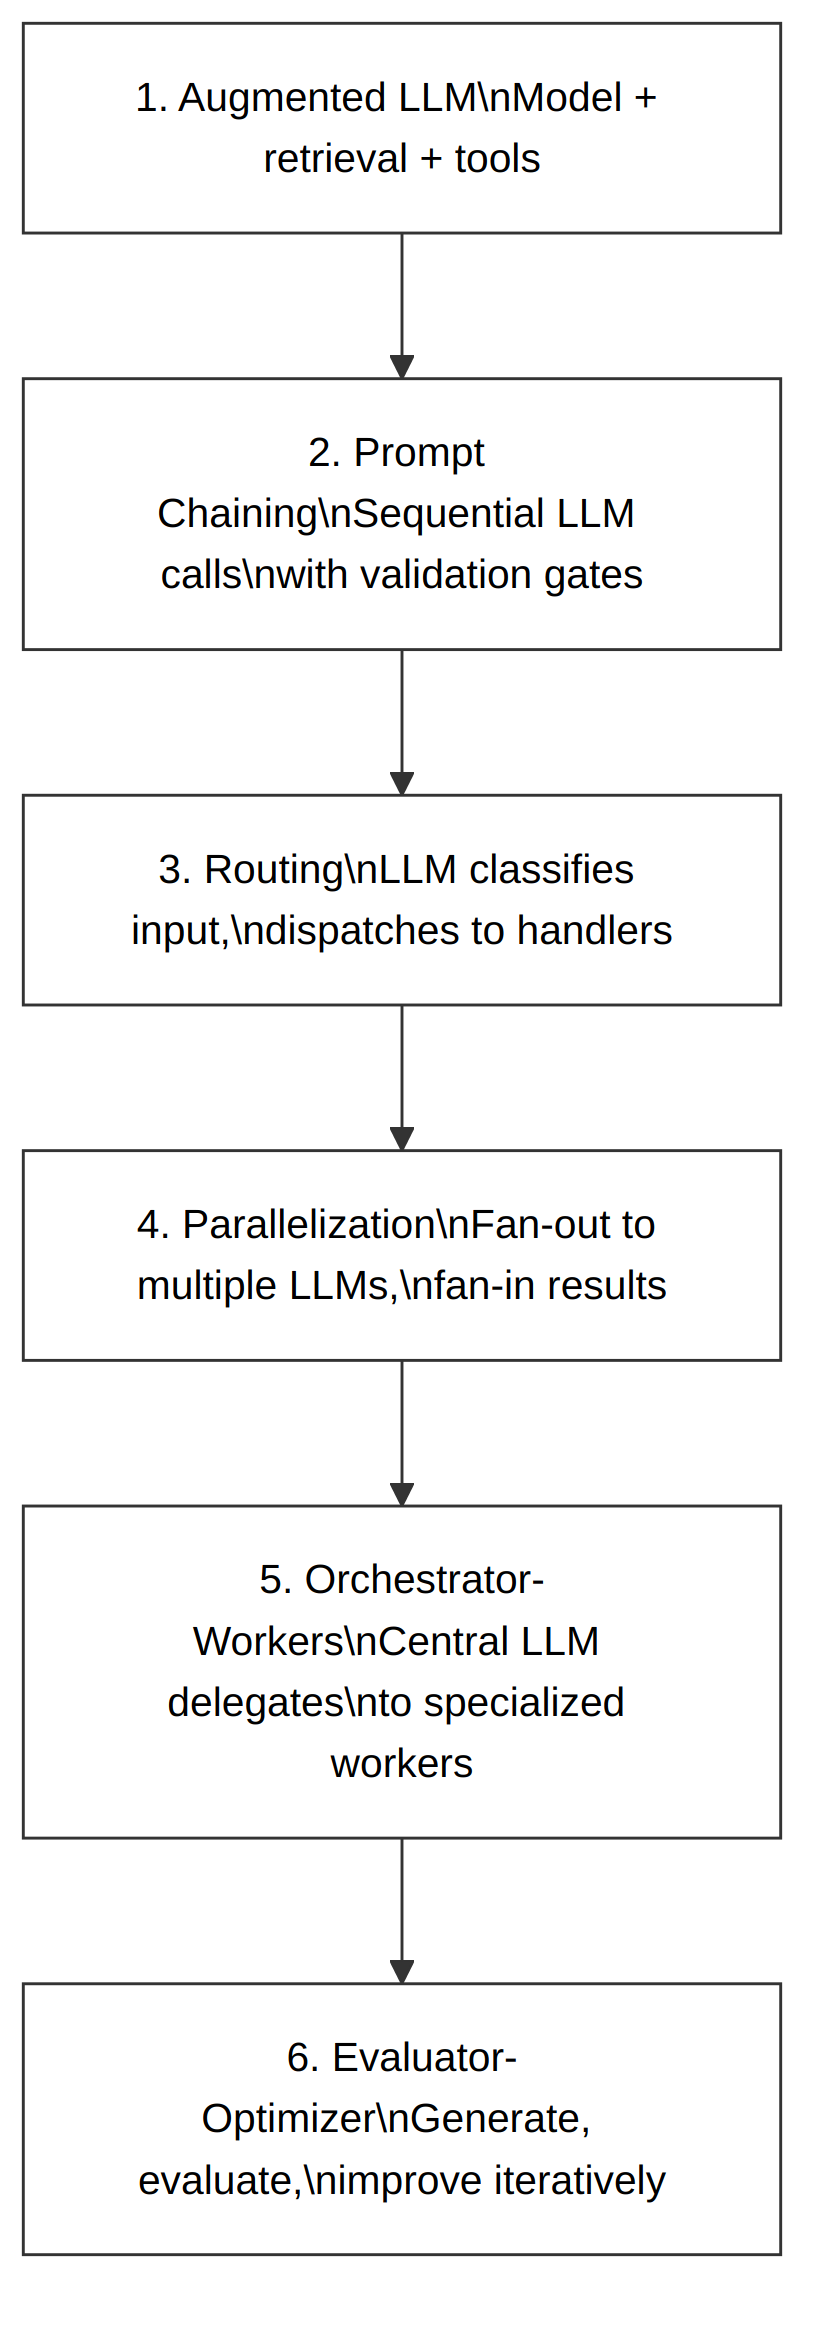
\includegraphics[width=0.85\textwidth,height=\textheight]{figures/diagram_3.png}
\caption{Figure 3. Anthropic's six composable patterns, arranged by
complexity. Green patterns (1--3) are workflows --- the developer
controls the flow. Amber patterns (4--5) introduce dynamic coordination.
The red pattern (6) involves the model evaluating its own output, which
requires careful design to avoid self-deception}
\end{figure}

\textbf{Pattern 1: Augmented LLM.} The foundation. A language model
enhanced with retrieval (access to a knowledge base) and tools (ability
to call external functions). This is not an agent --- the model responds
to a single request --- but it is the building block from which agents
are constructed.

\textbf{Pattern 2: Prompt chaining.} A sequence of LLM calls where each
call processes the output of the previous one. The critical feature is
\emph{gating}: between each step, a validation check determines whether
the output is acceptable before passing it to the next step. If the
output fails validation, the chain can retry or route to a fallback.
This is still a workflow --- the sequence is predetermined --- but it
handles multi-step tasks more reliably than a single large prompt.

\textbf{Pattern 3: Routing.} The LLM examines an input and classifies it
into one of several categories, then the system routes the input to a
specialized handler for that category. This is particularly effective
for systems that handle diverse request types --- a customer support
system that routes billing questions to one pipeline, technical issues
to another, and general inquiries to a third. The routing decision uses
the LLM's judgment, but the subsequent handling is deterministic.

\textbf{Pattern 4: Parallelization.} Multiple LLMs process the same
input simultaneously, and their outputs are aggregated. This is useful
for tasks where multiple perspectives improve quality --- having three
models independently analyze a document and then combining their
findings, or running the same analysis with different prompts and taking
the consensus. The cost is proportional to the number of parallel calls.

\textbf{Pattern 5: Orchestrator-Workers.} A central LLM (the
orchestrator) examines a task, decomposes it into sub-tasks, and
delegates each sub-task to a specialized worker. This is where the
system begins to exhibit true agent behavior, because the orchestrator
decides at runtime how to decompose the task. The delegation is dynamic
--- the orchestrator might send a research question to a search worker,
then based on the results, decide to send a follow-up to a different
worker.

\textbf{Pattern 6: Evaluator-Optimizer.} The system generates an output,
then a separate evaluation step assesses the quality of that output. If
the evaluation indicates deficiencies, the system revises and tries
again. This pattern is powerful but dangerous: without an external
ground truth (like a test suite), the evaluator is grading its own
homework. The Reflexion architecture (Shinn et al., 2023) demonstrated
an eighteen-percent accuracy improvement using this pattern, but the
improvement was contingent on having a reliable external evaluation
signal.

Anthropic's own recommendation is worth quoting directly: ``The most
successful implementations weren't using complex frameworks or
specialized libraries --- they were building with simple, composable
patterns'' (Anthropic, 2024).

\hypertarget{the-react-loop}{%
\subsubsection{3.2 The ReAct Loop}\label{the-react-loop}}

The most widely used agent architecture is ReAct --- Reason plus Act ---
introduced by Yao et al.~(2023). The agent alternates between thinking
about what to do next and taking an action, creating a cycle that
continues until the task is complete or a stopping condition is reached.

\begin{figure}
\centering
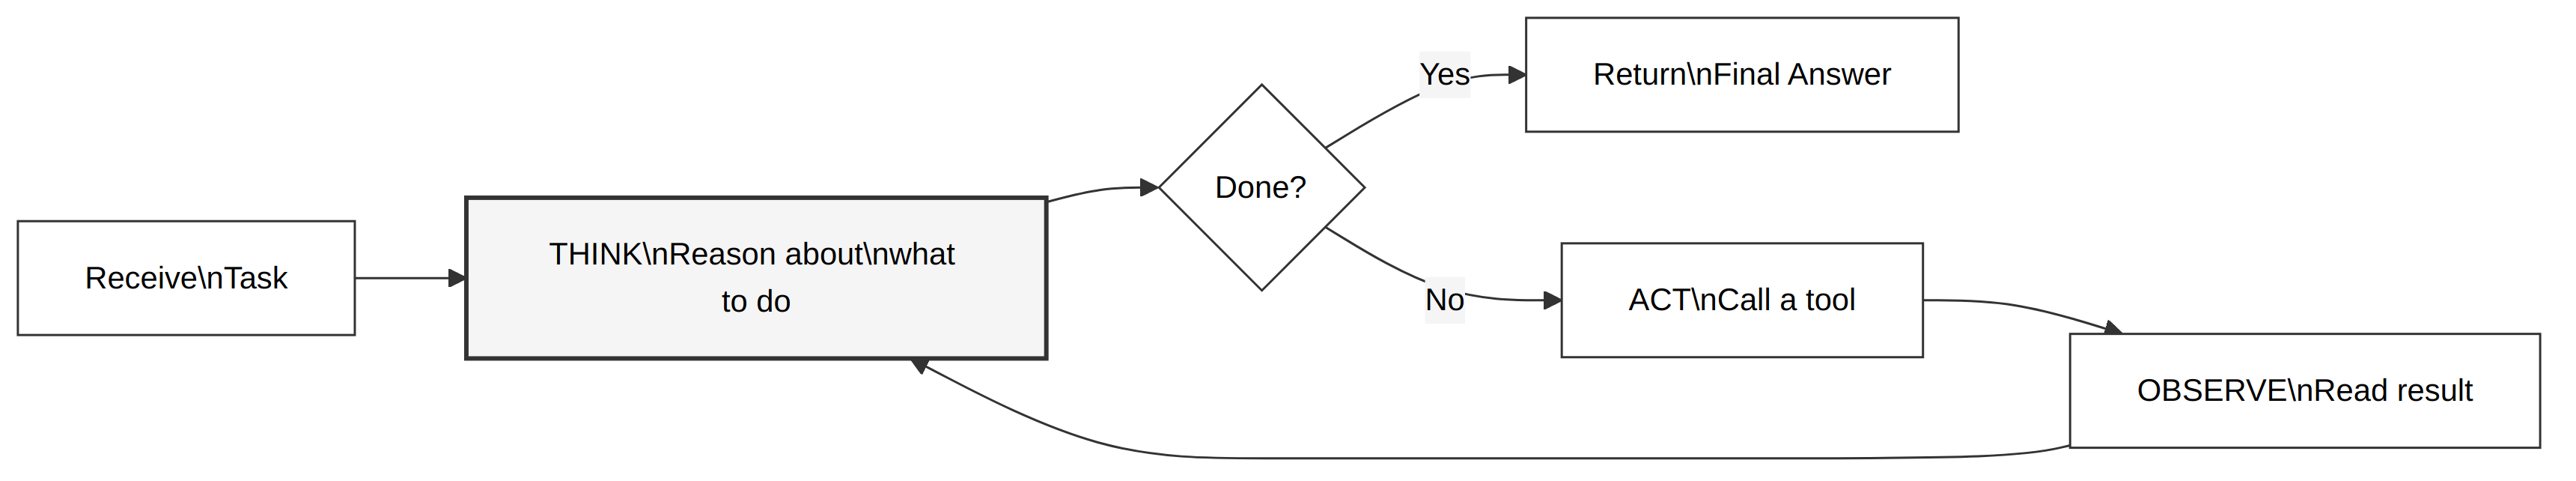
\includegraphics[width=0.85\textwidth,height=\textheight]{figures/diagram_4.png}
\caption{Figure 4. The ReAct loop. The agent thinks about the current
state, decides on an action, executes it, observes the result, and
repeats until it has enough information to answer or hits a stopping
condition}
\end{figure}

Each iteration of the loop follows three phases:

\textbf{Think.} The model examines the current state --- the original
task, the conversation history, and the results of any previous actions
--- and reasons about what to do next. In practice, this reasoning is
generated as text that appears in the model's output, making the agent's
decision process transparent and debuggable.

\textbf{Act.} Based on its reasoning, the model selects a tool and
provides arguments. For our research agent, the available tools might
include \passthrough{\lstinline!search\_papers!} (query arXiv),
\passthrough{\lstinline!read\_paper!} (fetch and parse a specific
paper), and \passthrough{\lstinline!write\_summary!} (save findings to a
file). The tool executes and returns a result.

\textbf{Observe.} The tool's result is added to the conversation, and
the cycle returns to the Think phase. The model now has new information
and can decide whether to take another action or provide a final answer.

\hypertarget{when-react-works-well}{%
\paragraph{When ReAct Works Well}\label{when-react-works-well}}

ReAct is well-suited to tasks that require \textbf{dynamic tool
selection across three to seven steps} where the next action depends on
the result of the previous one. A research agent that searches, reads
what it finds, and then decides whether to search again is a natural fit
for ReAct. The pattern's strength is flexibility: the agent can adapt
its approach based on what it discovers.

\hypertarget{when-react-fails}{%
\paragraph{When ReAct Fails}\label{when-react-fails}}

ReAct has three characteristic failure modes that practitioners should
anticipate:

\textbf{Myopic reasoning.} The agent optimizes for the next step without
considering the overall plan. It might find an interesting tangent in
step three and follow it for six more steps, losing sight of the
original objective. This is analogous to depth-first search without
backtracking --- locally productive, globally wasteful.

\textbf{Error propagation.} If the agent makes a wrong tool call in step
two --- selecting the wrong search terms, for example --- every
subsequent step operates on a flawed foundation. Unlike a workflow where
each step can be tested independently, ReAct errors compound through the
chain.

\textbf{Infinite loops.} Without an explicit circuit breaker\footnote{A
  \textbf{circuit breaker} is a mechanism that stops an agent after a
  predetermined number of steps, amount of time, or dollar cost. It
  prevents runaway execution. The term is borrowed from electrical
  engineering, where a circuit breaker prevents excessive current from
  damaging equipment.}, an agent can cycle indefinitely --- searching,
not finding what it needs, searching again with slightly different
terms, not finding it, and repeating. The \$47,000 API bill mentioned in
the introduction was generated by exactly this failure mode: two agents
in a ReAct loop talking to each other with no termination condition.

The circuit breaker is non-negotiable. Every ReAct implementation must
include a maximum iteration count, and reaching that limit should
produce a graceful summary of progress rather than an error.

\hypertarget{our-running-example-as-a-react-agent}{%
\paragraph{Our Running Example as a ReAct
Agent}\label{our-running-example-as-a-react-agent}}

Here is what our research agent looks like when upgraded from a Level 1
cron job to a Level 5 ReAct agent:

\begin{lstlisting}[language=Python]
# research_agent.py -- ReAct loop with circuit breaker
from tools import search_papers, read_paper, write_summary

SYSTEM_PROMPT = """You are a research assistant. Given a research question,
search for relevant papers, read the most promising ones, and write a summary
of your findings. Use the available tools to gather information. When you have
enough information to write a comprehensive summary, do so and stop."""

def react_loop(question: str, max_iterations: int = 10) -> str:
    messages = [
        {"role": "system", "content": SYSTEM_PROMPT},
        {"role": "user", "content": question}
    ]

    for step in range(max_iterations):
        response = llm.chat(messages, tools=[search_papers, read_paper, write_summary])

        if response.has_tool_call:
            tool_name = response.tool_call.name
            tool_args = response.tool_call.arguments
            result = execute_tool(tool_name, tool_args)
            messages.append({"role": "tool", "content": result})
        else:
            return response.text  # Final answer

    return "Reached maximum iterations. Here is what I found so far: ..."
\end{lstlisting}

The critical difference from the cron job version is that the agent
\emph{decides} what to search for, \emph{decides} which papers to read,
and \emph{decides} when it has enough information. The human provides
the question; the agent provides the methodology. This flexibility is
the reason to use an agent --- and it is also the reason that evaluation
(Chapter 6) becomes essential, because the agent's choices are no longer
predetermined.

\hypertarget{plan-and-execute}{%
\subsubsection{3.3 Plan-and-Execute}\label{plan-and-execute}}

For tasks with more than about seven steps, the ReAct pattern's myopic
reasoning becomes a liability. The alternative is to separate planning
from execution: first create a plan, then execute it step by step,
revising the plan if new information makes it obsolete.

\begin{figure}
\centering
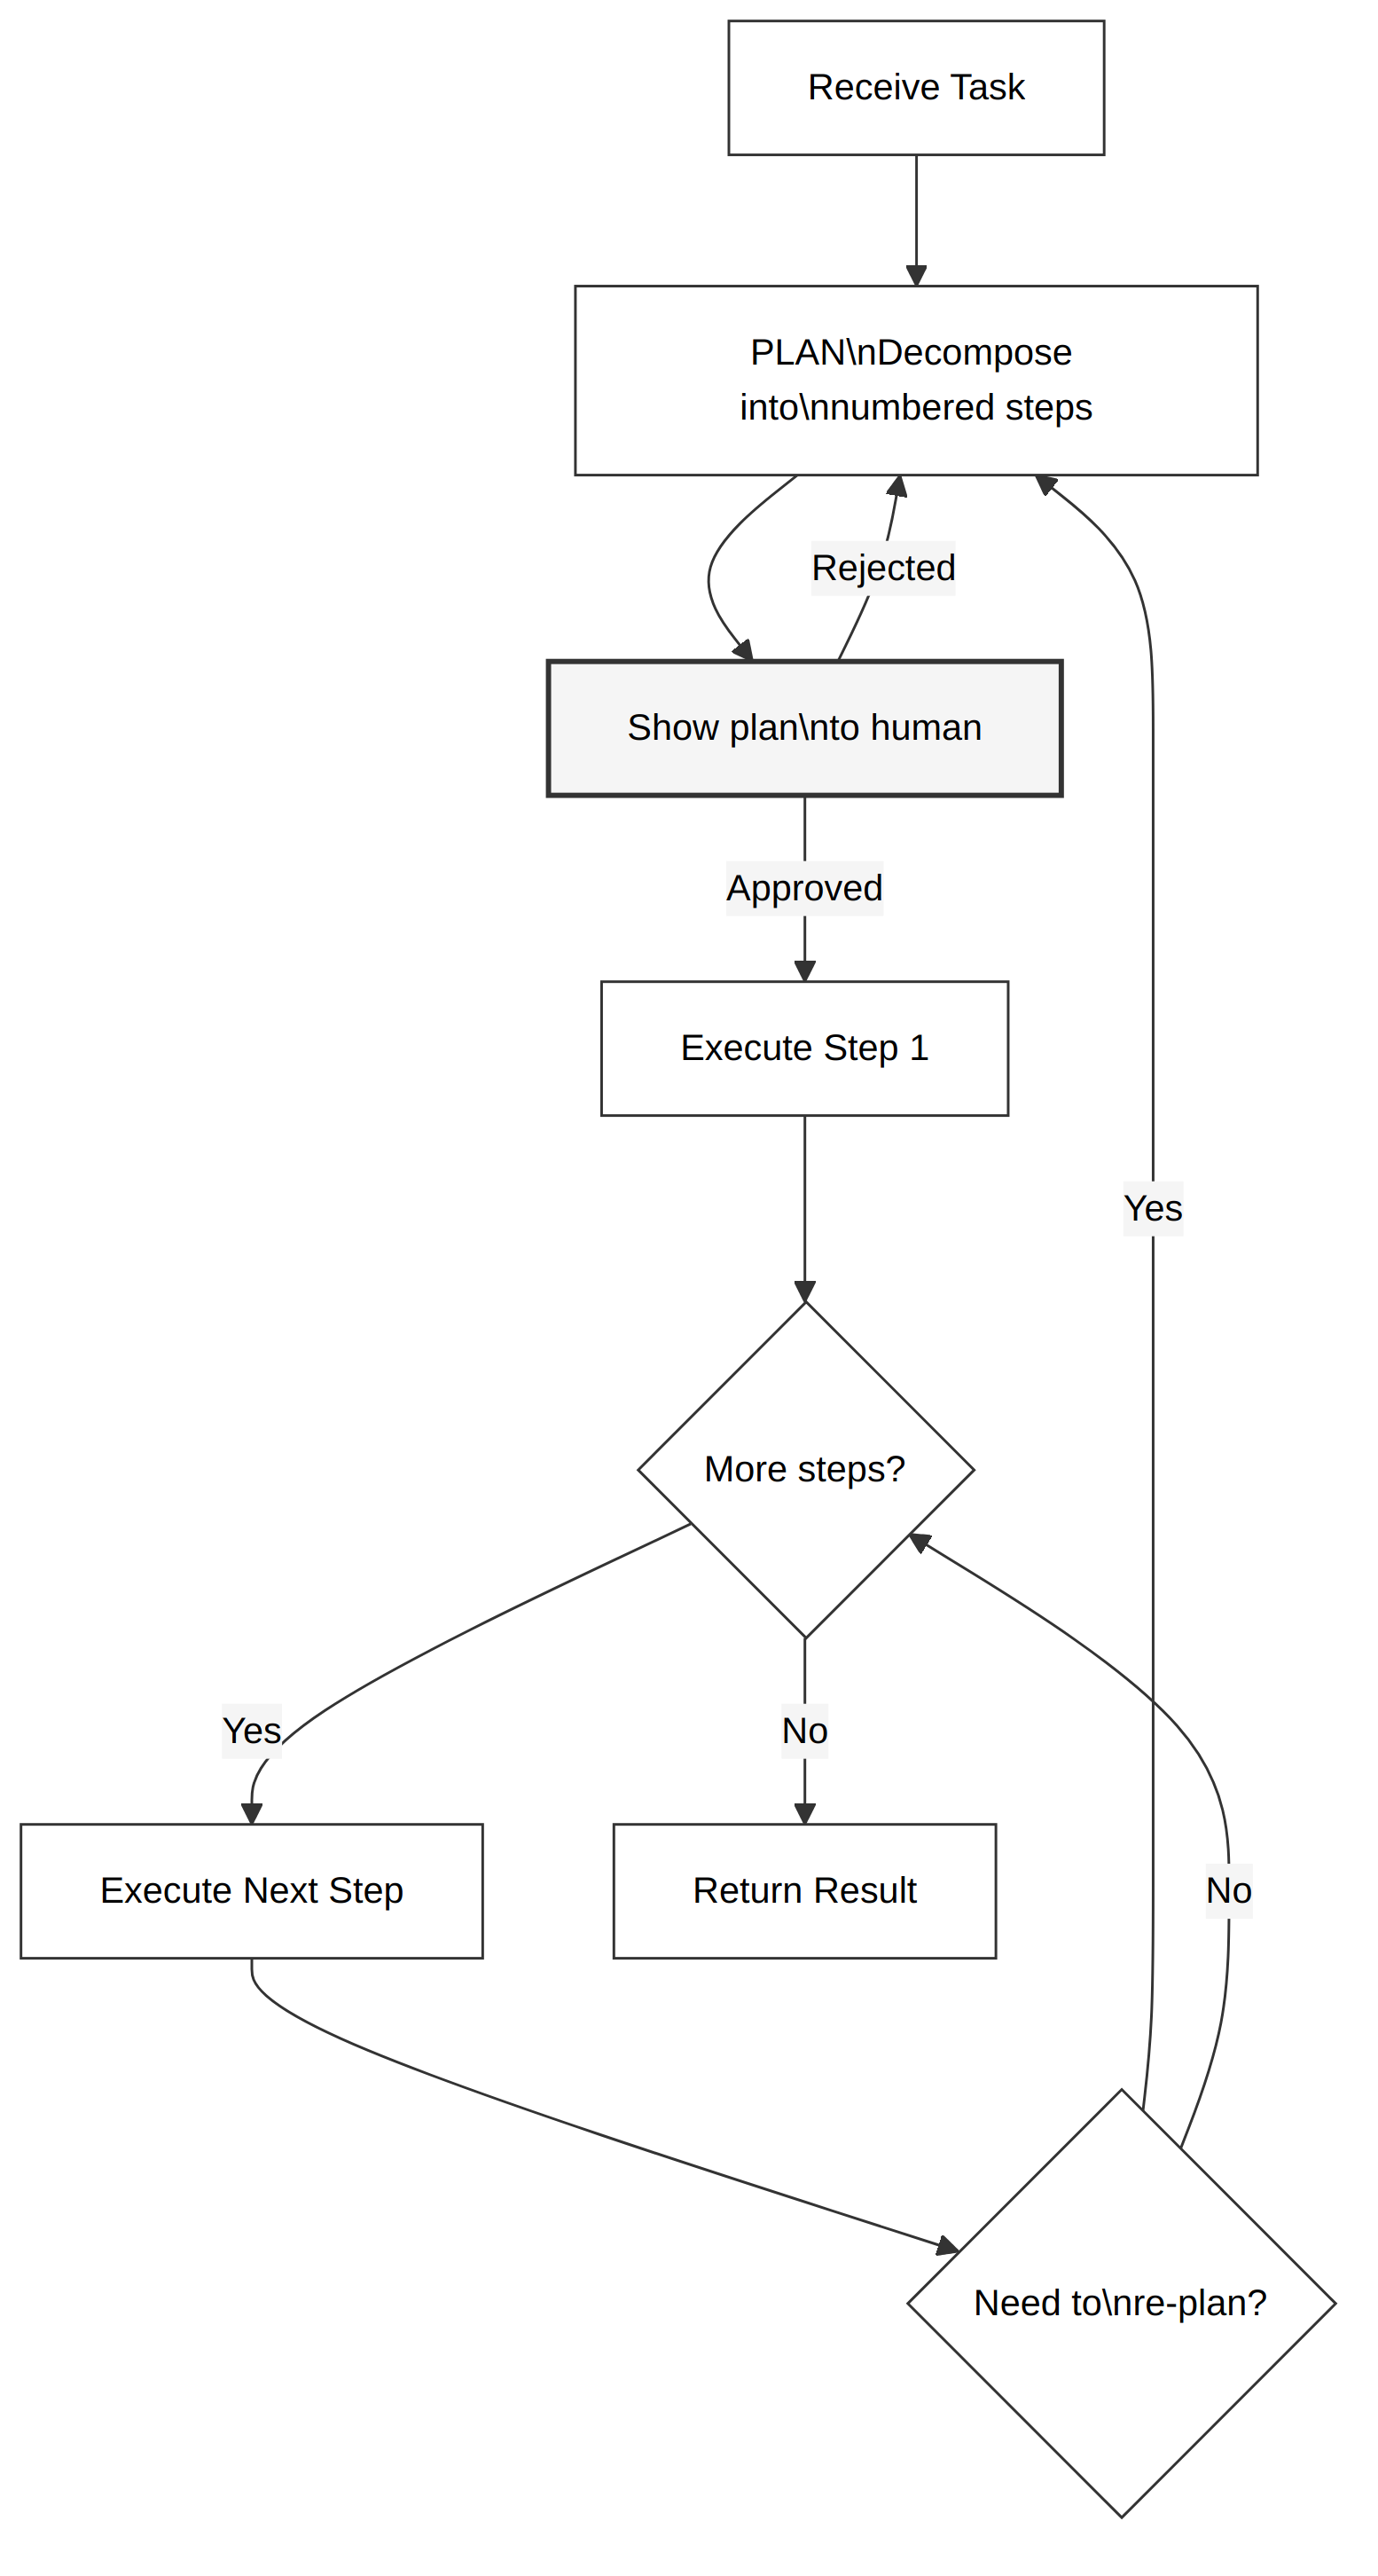
\includegraphics[width=0.85\textwidth,height=\textheight]{figures/diagram_5.png}
\caption{Figure 5. The Plan-and-Execute architecture. The planning phase
produces a numbered list of steps. An optional human review gate (amber)
allows approval or rejection of the plan before execution begins. During
execution, the agent can trigger re-planning if it discovers that the
original plan is no longer viable}
\end{figure}

This architecture has two important advantages over ReAct. First, the
planning step provides a \textbf{human review opportunity} --- the user
can examine the plan, reject it, or modify it before any actions are
taken. This is both a safety mechanism and a debugging tool: if the plan
looks wrong, you know before any work is done. Second, the explicit plan
helps the agent maintain coherence over long task sequences, because
each step has a clear relationship to the overall objective.

The trade-off is \textbf{plan rigidity}. Real tasks often reveal
information that changes the plan --- a paper that opens an unexpected
line of inquiry, an API that returns data in a different format than
expected. The re-planning mechanism (the ``Need to re-plan?'' decision
in Figure 5) addresses this, but re-planning is expensive: it requires
another LLM call to analyze the current state and produce a revised
plan.

Claude Code, Anthropic's command-line coding tool, uses a
plan-and-execute architecture. When asked to make changes across
multiple files, it first generates a plan listing the files to modify
and the nature of each change, then executes the plan sequentially. The
plan is visible to the user, serving as both a transparency mechanism
and an implicit approval gate.

\hypertarget{the-minimal-agent-philosophy}{%
\subsubsection{3.4 The Minimal Agent
Philosophy}\label{the-minimal-agent-philosophy}}

At the opposite end of the complexity spectrum from multi-agent
frameworks lies a provocative position articulated by Mario Zechner,
creator of the PI coding agent, and Armin Ronacher, creator of Flask and
co-founder of Sentry. Their argument: \textbf{four tools are enough.}

PI's entire tool set consists of: - \textbf{Read} --- read a file with
optional offset and limit for large files - \textbf{Write} --- create or
overwrite a file, creating parent directories automatically -
\textbf{Edit} --- precise text replacement within a file - \textbf{Bash}
--- execute a shell command synchronously

That is it. No web search tool, no database query tool, no specialized
API integrations. If the agent needs to search the web, it writes a curl
command and executes it through Bash. If it needs to query a database,
it writes a SQL command and pipes it through the database client. The
tools the model already knows from its training data --- bash commands,
curl, git, python --- become the universal interface.

Zechner's argument rests on three observations (Zechner, 2025):

\textbf{Frontier models already understand standard tools.} Models are
trained on vast amounts of code that uses bash, curl, git, and other
command-line tools. They do not need a specialized ``web search'' tool
with a custom JSON schema --- they know how to write
\passthrough{\lstinline!curl https://api.example.com/search?q=...!} and
parse the result. Providing a specialized tool adds cognitive overhead
(the model must learn the tool's specific interface) without adding
capability.

\textbf{System prompt size inversely correlates with performance.} PI's
system prompt is approximately 500 tokens. Competing agents use 10,000
or more. Zechner's observation, supported by his experience building and
testing PI, is that massive system prompts add noise rather than signal.
The model's attention is finite; burying critical instructions in a sea
of tool descriptions dilutes them.

\textbf{Every tool description consumes context.} The math is
straightforward. Four tools at approximately 200 tokens per description
consume 800 tokens of context. Forty tools consume 8,000 tokens. At the
upper extreme, Zechner measured that MCP\footnote{\textbf{MCP} (Model
  Context Protocol) is a standard for connecting AI models to external
  tools, developed by Anthropic and now governed by the Linux
  Foundation. It provides a uniform interface for tool definitions,
  similar to how USB provides a uniform interface for hardware
  peripherals.} tool descriptions consumed seven to nine percent of the
context window regardless of whether those tools were used --- a
permanent tax on every API call.

This philosophy is validated by benchmark data. Zechner conducted 120
controlled tests comparing CLI-based tool use against MCP-based
equivalents. The results showed identical success rates (100\% across
all conditions) but CLI tools were twenty to twenty-nine percent cheaper
per task due to lower token consumption (Zechner, 2025b).

The Vercel experiment provides additional evidence. Vercel's data agent,
d0, initially had dozens of specialized tools. The team removed eighty
percent of them. The result was counterintuitive: the success rate
increased from eighty to one hundred percent, with fewer steps, fewer
tokens, and faster responses. The removed tools had been solving
problems that the model could handle natively --- the team had
overestimated the value of specialized tools and underestimated the cost
of tool description overhead (Vercel, 2025).

The minimalist position is not universally correct. Some tasks genuinely
require tools that cannot be synthesized from bash --- authenticated API
calls to proprietary services, GUI interaction, or specialized hardware
control. But the principle is powerful as a default: \textbf{before
adding a tool, ask whether a bash script would suffice.} If it would,
the bash script is better --- it costs zero context tokens until
invoked, it is composable with other scripts, and the model already
knows how to use it.

\hypertarget{the-hybrid-pattern-deterministic-steps-with-llm-decision-nodes}{%
\subsubsection{3.5 The Hybrid Pattern: Deterministic Steps with LLM
Decision
Nodes}\label{the-hybrid-pattern-deterministic-steps-with-llm-decision-nodes}}

Between the fully autonomous agent and the fully deterministic workflow
lies a pattern that deserves far more attention than it receives. The
hybrid pattern embeds one or more LLM decision nodes within an otherwise
deterministic pipeline.

\begin{figure}
\centering
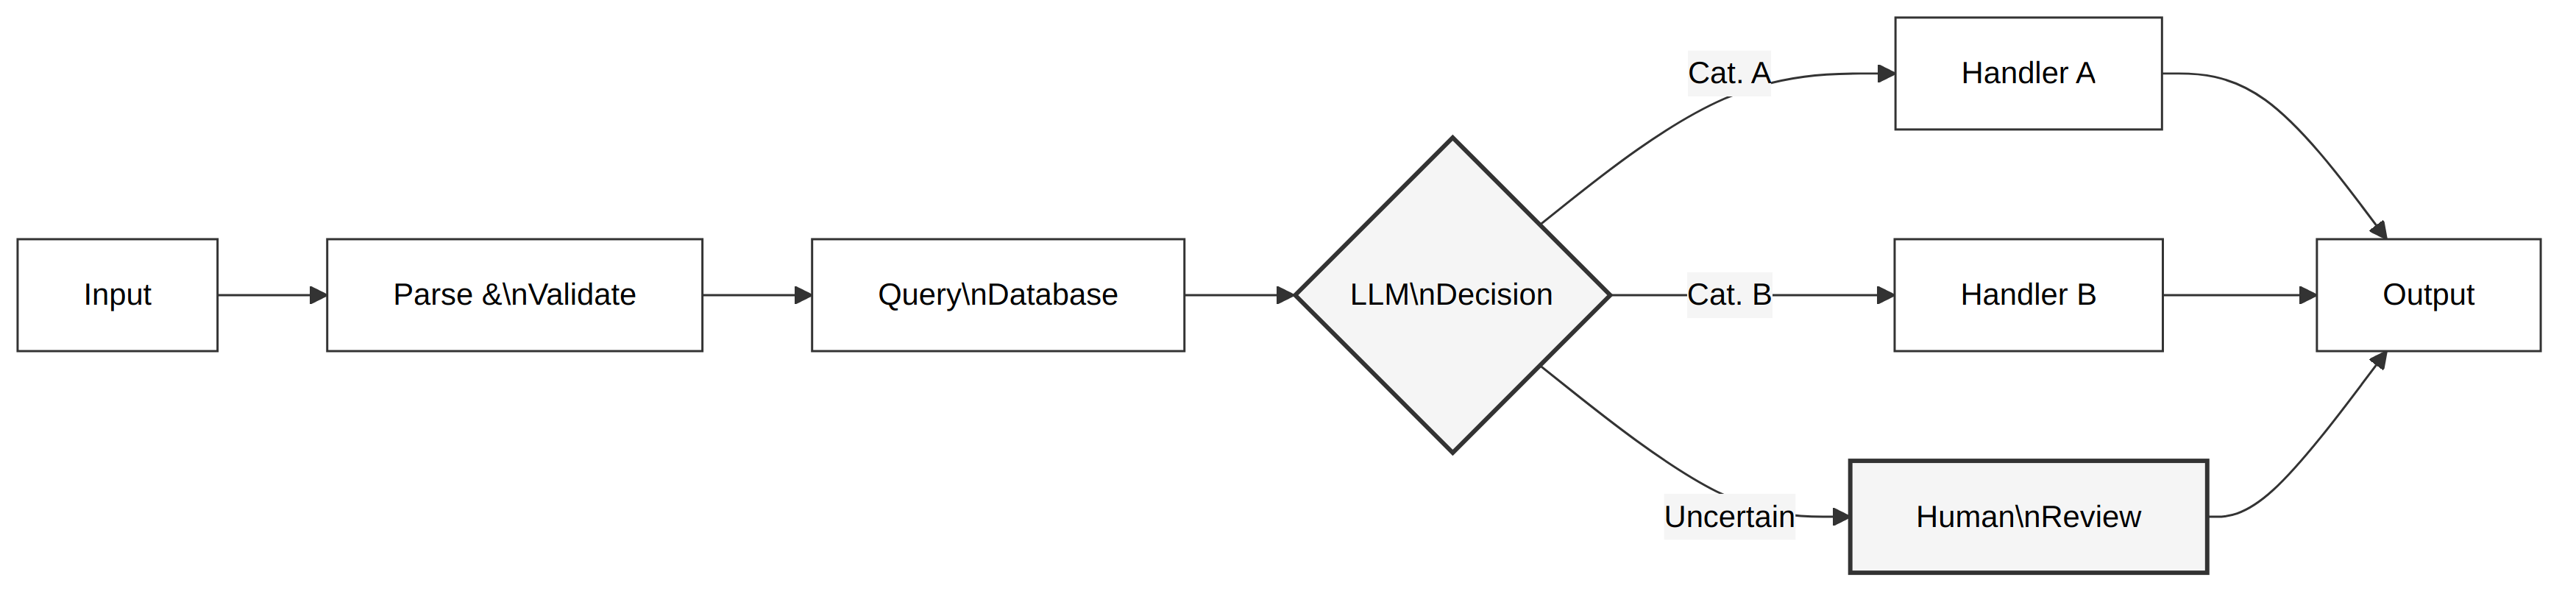
\includegraphics[width=0.85\textwidth,height=\textheight]{figures/diagram_6.png}
\caption{Figure 6. The hybrid pattern. The pipeline is deterministic
except for one decision node (amber) where the LLM classifies the input.
Uncertain classifications route to human review (blue). This pattern
combines workflow reliability with AI flexibility at the single point
where flexibility is needed}
\end{figure}

The hybrid pattern is, in the author's experience, the most undervalued
approach in the entire AI automation landscape. It earns a
hype-versus-reality score of +4: the reality exceeds the hype, because
nobody writes blog posts about it. It is the boring thing that actually
works.

Three concrete implementations illustrate the pattern's versatility:

\textbf{Classification node.} An incoming document (email, support
ticket, medical record) arrives at the pipeline. The LLM examines it and
assigns it to one of N predefined categories. The remainder of the
pipeline is determined by the category --- routing, processing, response
template, escalation rules. The LLM's output space is constrained to the
category set, which makes it both more reliable and easier to validate.

\textbf{Extraction node.} An unstructured document enters the pipeline.
The LLM extracts structured fields --- names, dates, amounts, reference
numbers --- and outputs them in a defined schema. The pipeline validates
the extracted fields against the schema, rejecting malformed results,
and processes the validated data through deterministic steps.

\textbf{Decision node with confidence routing.} The LLM evaluates a case
and provides both a decision and a confidence score. Cases above the
confidence threshold proceed autonomously; cases below it route to a
human reviewer. This creates a natural feedback loop: the human
decisions on uncertain cases can be used to improve the model over time.

\hypertarget{harness-engineering-why-the-scaffold-matters-more-than-the-model}{%
\subsubsection{3.6 Harness Engineering: Why the Scaffold Matters More
Than the
Model}\label{harness-engineering-why-the-scaffold-matters-more-than-the-model}}

Daniel Miessler, through his CraftersLab research, argues that 2026 is
``the year of harnesses'' --- the year when the engineering community
recognizes that the infrastructure around the model matters more than
the model itself (Miessler, 2026).

The evidence supports this claim. The EPIC-S benchmark evaluated agents
across five dimensions (Efficiency, Planning, Initiative, Correctness,
Safety) and found that only twenty-four percent succeeded across all
criteria. The failures were overwhelmingly architectural --- incorrect
tool use, missing safety controls, poor context management --- not model
limitations. Switching from one frontier model to another rarely changed
the outcome. Changing the harness --- the tools, the prompts, the error
handling, the evaluation pipeline --- changed everything.

Ronacher articulates the same principle from a practitioner's
perspective: ``The differences between models are significant enough
that you will need to build your own agent abstraction'' (Ronacher,
2025). His advice is to work directly with model-provider SDKs (the
OpenAI or Anthropic Python libraries) rather than abstraction layers
like the Vercel AI SDK. The abstractions, he argues, hide
provider-specific behaviors that matter for agent reliability --- and
when they break, they break in ways that are difficult to diagnose.

This leads to a principle that will recur throughout this manual:
\textbf{Scaffolding \textgreater{} Models (80/20).} Eighty percent of an
agent system's production value comes from its scaffolding --- the tool
definitions, the error handling, the context management, the evaluation
infrastructure, the cost controls. Twenty percent comes from the
underlying model. An Opus-level model with poorly written tool
descriptions will underperform a Haiku-level model with excellent tool
descriptions. Invest accordingly.

\begin{center}\rule{0.5\linewidth}{0.5pt}\end{center}

\hypertarget{context-engineering-managing-what-the-model-sees}{%
\subsection{4. Context Engineering: Managing What the Model
Sees}\label{context-engineering-managing-what-the-model-sees}}

If you read only one chapter of this manual, read this one. Context
engineering --- the discipline of controlling what information the model
has access to at each step --- is where most agent failures originate
and where most performance improvements are found. It is not an
optimization technique; it is a fundamental design discipline.

\hypertarget{why-context-engineering-exists}{%
\subsubsection{4.1 Why Context Engineering
Exists}\label{why-context-engineering-exists}}

The term ``context engineering'' emerged in mid-2025 when Shopify CEO
Tobi Lutke reframed ``prompt engineering'' as insufficient for
describing the actual skill involved in building production AI systems.
Andrej Karpathy co-signed the reframing: ``In every industrial-strength
LLM app, context engineering is the delicate art and science of filling
the context window with just the right information for the next step''
(Karpathy, 2025).

The reframing is more than semantic. The prompt --- the instruction you
give the model --- is approximately five percent of the context window.
The other ninety-five percent consists of retrieved documents,
conversation history, tool definitions, intermediate results from
previous steps, and various forms of state. If you spend all your
optimization effort on the five percent (writing a better prompt) while
ignoring the ninety-five percent (what documents are retrieved, what
conversation history is included, how your tools are described), you are
optimizing the wrong thing.

Anthropic's own data quantifies this: context engineering strategies
yield \textbf{fifty-four percent better agent performance} compared to
prompt optimization alone (Anthropic, 2025a).

Three forces make context engineering non-trivial for agents:

\textbf{Context rot.} As tokens accumulate in the context window, model
performance degrades. This is not merely a theoretical concern. Zechner
reports that ``things start falling apart around 100K tokens. Benchmarks
be damned'' (Zechner, 2025). Academic research confirms a ``lost in the
middle'' effect where information placed in the center of a long context
is recalled less accurately than information at the beginning or end.
For agents that run for dozens of steps, each adding tool outputs to the
context, this degradation is progressive and cumulative.

\textbf{Token explosion.} Production agents consume tokens at rates that
surprise even experienced practitioners. Manus, a commercially deployed
agent platform, reports a 100:1 input-to-output token ratio in
production (Manus, 2025). A fifty-step agent session can easily
accumulate 200,000 or more tokens of context, most of which consists of
stale tool outputs from early steps that are no longer relevant.

\textbf{Cost scaling.} Every token in the context window is paid for at
\emph{every} API call. A 200,000-token context costs the same whether
those tokens are actively contributing to the model's reasoning or
sitting unused as dead weight from step three of a twenty-step process.
This cost accumulates across calls: by the tenth step, you have paid for
those dead-weight tokens ten times.

The solutions fall into four categories, which this chapter covers in
sequence: \textbf{Offload} (move state out of the context window into
files), \textbf{Reduce} (compress what remains in context),
\textbf{Isolate} (give sub-tasks fresh context windows), and
\textbf{Disclose progressively} (load information on demand rather than
upfront).

\hypertarget{offload-the-file-system-as-external-memory}{%
\subsubsection{4.2 Offload: The File System as External
Memory}\label{offload-the-file-system-as-external-memory}}

The most underappreciated context management technique is also the
simplest: write information to files and read it back when needed. The
file system has unlimited capacity, persists across sessions, and is
directly manipulable by the agent through standard file operations.

Zechner articulated the governing principle: ``Prompts are code,
.json/.md files are state'' (Zechner, 2025a). Instead of keeping the
agent's plan, progress, and decisions in the conversation history ---
where they consume tokens at every step and are vulnerable to context
truncation --- write them to disk. The file is the ground truth. The
model ``remembers'' only what is written to disk and loaded into context
when needed.

\textbf{The PLAN.md pattern.} Instead of maintaining a plan in the
conversation, the agent writes a PLAN.md file to disk. Each step is
listed with its status (pending, in progress, completed). When the agent
begins a new step, it reads PLAN.md, identifies the next pending step,
executes it, updates the file, and continues. The plan survives context
window compaction, session boundaries, and even process restarts. It is
observable (a human can read it at any time), version-controlled (git
tracks every change), and independent of any particular model or
framework.

\textbf{The todo recitation pattern.} Manus discovered a subtle but
powerful technique: having the agent periodically rewrite its todo list
at the \emph{end} of the context (Manus, 2025). The act of rewriting
forces the model to articulate its current objectives, which counteracts
goal drift --- the tendency of long-running agents to lose sight of the
original task as intermediate results accumulate. Placing the todo at
the end of the context exploits the recency bias\footnote{\textbf{Recency
  bias} in transformer models refers to the tendency for the model to
  pay more attention to tokens near the end of the context window than
  to tokens in the middle. This is a well-documented effect that
  influences both retrieval accuracy and instruction following.} that
all transformer models exhibit: information at the end of the context
receives disproportionately high attention.

\textbf{Recoverable offloading.} Manus's key insight is that context
compression must be \emph{recoverable}. When removing content from the
context to save tokens, always preserve enough metadata to re-fetch the
content if needed. Drop a web page's content but keep the URL. Drop a
file's content but keep the file path. Drop a search result's details
but keep the search query that produced it. This way, if the model later
needs the information, it can retrieve it through a tool call rather
than having lost it permanently.

\hypertarget{our-running-example-with-file-based-state}{%
\paragraph{Our Running Example with File-Based
State}\label{our-running-example-with-file-based-state}}

Here is how our research agent evolves to use file-based state
management:

\begin{lstlisting}[language=Python]
# research_agent_v2.py -- with file-based state
from pathlib import Path
import json

STATE_FILE = Path("research_state.md")
FINDINGS_FILE = Path("findings.jsonl")

def save_state(phase, searched_queries, read_papers, pending_papers):
    """Write agent state to disk -- survives context resets."""
    state = f"""# Research State
## Phase: {phase}
## Searched Queries
{chr(10).join(f'- [x] {q}' for q in searched_queries)}
## Papers Read
{chr(10).join(f'- [x] {p}' for p in read_papers)}
## Papers Pending
{chr(10).join(f'- [ ] {p}' for p in pending_papers)}
"""
    STATE_FILE.write_text(state)

def append_finding(finding: dict):
    """Append a finding to the episodic log -- never loses data."""
    with open(FINDINGS_FILE, "a") as f:
        f.write(json.dumps(finding) + "\n")
\end{lstlisting}

The agent now has two persistent artifacts: a state file that tracks its
progress and a findings log that accumulates results. If the context
window is compacted or the session ends, the agent can resume by reading
these files --- it does not depend on conversation history for
continuity.

\hypertarget{reduce-compaction-summarization-and-filtering}{%
\subsubsection{4.3 Reduce: Compaction, Summarization, and
Filtering}\label{reduce-compaction-summarization-and-filtering}}

When context grows beyond what can be offloaded, the remaining content
must be compressed. Three techniques apply, from simplest to most
aggressive.

\textbf{Sliding window compaction} replaces old messages with summaries
while keeping recent messages in full detail. Google's ADK framework
implements this natively: every N conversation turns, the system
summarizes the older turns using a cheap, fast model (like Claude Haiku)
and keeps only the most recent turns in their original form. This
maintains a roughly constant context size regardless of conversation
length. Manus reports maintaining agent quality over fifty or more tool
calls with sixty to eighty percent token reduction using this technique
(Manus, 2025).

The critical design decision is the \textbf{overlap parameter} --- how
many recent messages to keep verbatim. Too few, and the model loses
thread of the immediate conversation. Too many, and the compaction
savings are negligible. In practice, keeping the two to three most
recent exchanges verbatim, plus a summary of everything prior, works
well for most agent tasks.

\textbf{Tool output compaction} addresses the largest source of context
bloat. A single \passthrough{\lstinline!git diff!} command can produce
10,000 tokens of output when only 200 tokens contain actionable
information. A web search might return full page content when only the
snippets are needed for the current reasoning step. The solution is to
compress tool outputs before adding them to the context, preserving key
data (error messages, file paths, URLs, numerical values) while
discarding verbose detail.

Manus's principle applies here: compression must be recoverable. After
compacting a web page to a brief summary, append the note: ``{[}Full
content available at URL --- re-fetch if needed{]}.'' This way, the
agent can retrieve the full content if its summarized form proves
insufficient.

\textbf{Relevance-based filtering} is the most aggressive technique.
Before each LLM call, score each message in the context by its relevance
to the current task and drop the lowest-scoring items. Always retain
certain categories of messages regardless of relevance: the system
prompt, the most recent exchanges, and any messages containing error
information. This technique can dramatically reduce context size but
carries a risk of dropping information that turns out to be relevant in
unexpected ways.

\hypertarget{isolate-sub-agents-with-fresh-context}{%
\subsubsection{4.4 Isolate: Sub-Agents with Fresh
Context}\label{isolate-sub-agents-with-fresh-context}}

For complex tasks that would overwhelm a single context window, the most
powerful technique is to spawn sub-agents that operate in their own
fresh context windows. The parent agent (the orchestrator) maintains a
lean context containing only the overall plan and high-level progress.
Each sub-agent receives a focused brief --- the specific sub-task
description, relevant configuration, and pointers to any state files ---
and works independently.

The GSD framework (26,000+ GitHub stars) implements this rigorously. The
orchestrator reads a state file (STATE.md) at the start of each session,
identifies the next task in the plan, and spawns a sub-agent with only
the task description and relevant project configuration. The sub-agent
cannot see the orchestrator's conversation history, other tasks'
results, or the full project state --- it sees only what it needs for
its specific task. When the sub-agent completes, it returns a summary to
the orchestrator. Not the full transcript. Not every intermediate step.
Just the summary.

This approach has two benefits. First, the orchestrator's context stays
lean --- typically ten to fifteen percent of the window --- leaving
ample room for ongoing work. Second, sub-agent failures are isolated. If
a sub-agent enters an unproductive loop or encounters an error, the
orchestrator's context is not polluted with pages of error messages. The
orchestrator receives a summary indicating that the sub-task failed, and
can decide how to proceed (retry, skip, escalate to human).

Ronacher adds a nuance to this pattern: when a sub-agent fails, the
\emph{what didn't work} information should be preserved even if the full
error trace is discarded (Ronacher, 2025). This prevents the
orchestrator from assigning the same doomed approach to a new sub-agent.

PI takes a different approach to isolation through \textbf{session
branching}. Instead of spawning separate processes, PI structures
sessions as trees rather than linear conversations. The user (or agent)
can branch the session, explore a sub-problem in the branch, and bring
only the result back to the main session. The full branch history
remains in the session file for debugging, but the main context sees
only the branch's conclusion.

\hypertarget{progressive-disclosure-loading-information-on-demand}{%
\subsubsection{4.5 Progressive Disclosure: Loading Information on
Demand}\label{progressive-disclosure-loading-information-on-demand}}

The final context management strategy is to load information only when
it is needed, rather than front-loading everything into the context at
the start of a session.

\textbf{The Vercel lesson.} As discussed in Section 3.4, Vercel
discovered that reducing their agent's tool set from dozens of tools to
a handful improved performance dramatically. The explanation lies in
progressive disclosure: each tool description consumes approximately 100
to 500 tokens of context, and those tokens are present at \emph{every}
API call regardless of whether the tool is used. With eighty tools
active, the model was spending significant reasoning capacity simply
deciding which tool to use --- a decision-making overhead that degraded
the quality of its actual task performance.

\textbf{Three-layer skill disclosure.} Anthropic's Agent Skills
framework implements progressive disclosure through three levels:

\begin{enumerate}
\def\labelenumi{\arabic{enumi}.}
\tightlist
\item
  \textbf{Metadata level} (approximately 50 tokens per skill): the
  skill's name and a one-line description. This layer is always loaded,
  giving the model awareness of available capabilities at minimal
  context cost.
\item
  \textbf{Instruction level} (approximately 500 tokens per skill): the
  skill's full instructions, including usage patterns and constraints.
  This layer loads only when the model decides to invoke the skill.
\item
  \textbf{Resource level} (variable size): scripts, templates, reference
  data, and other materials the skill needs. This layer loads only
  during skill execution.
\end{enumerate}

The result is that an agent can have hundreds of available skills at a
total context cost of approximately 5,000 tokens (metadata only),
loading full instructions for only the one or two skills relevant to the
current task.

\textbf{Tool masking versus tool removal.} Manus discovered a subtle
cache-related issue with dynamic tool management. Adding or removing
tools between conversation turns changes the system prompt, which
invalidates the KV cache\footnote{The \textbf{KV cache} (key-value
  cache) is an optimization used by transformer models to avoid
  recomputing attention over previously processed tokens. When the
  context changes --- even slightly, such as adding or removing a tool
  definition --- the cache may be partially or fully invalidated,
  requiring expensive recomputation. This is why context consistency
  matters for cost and latency.} and forces the model to reprocess the
entire context. Their solution: keep all tool definitions in the system
prompt at all times, but use logit masking to prevent the model from
selecting tools that are not appropriate for the current step. The
definitions stay in the cache; the model simply cannot choose masked
tools. Both goals --- context consistency and tool restriction --- are
met without cache invalidation.

\hypertarget{the-context-engineering-stack}{%
\subsubsection{4.6 The Context Engineering
Stack}\label{the-context-engineering-stack}}

The four strategies described in this chapter form a layered stack. Each
layer builds on the one below, and the order of implementation matters.

\begin{figure}
\centering
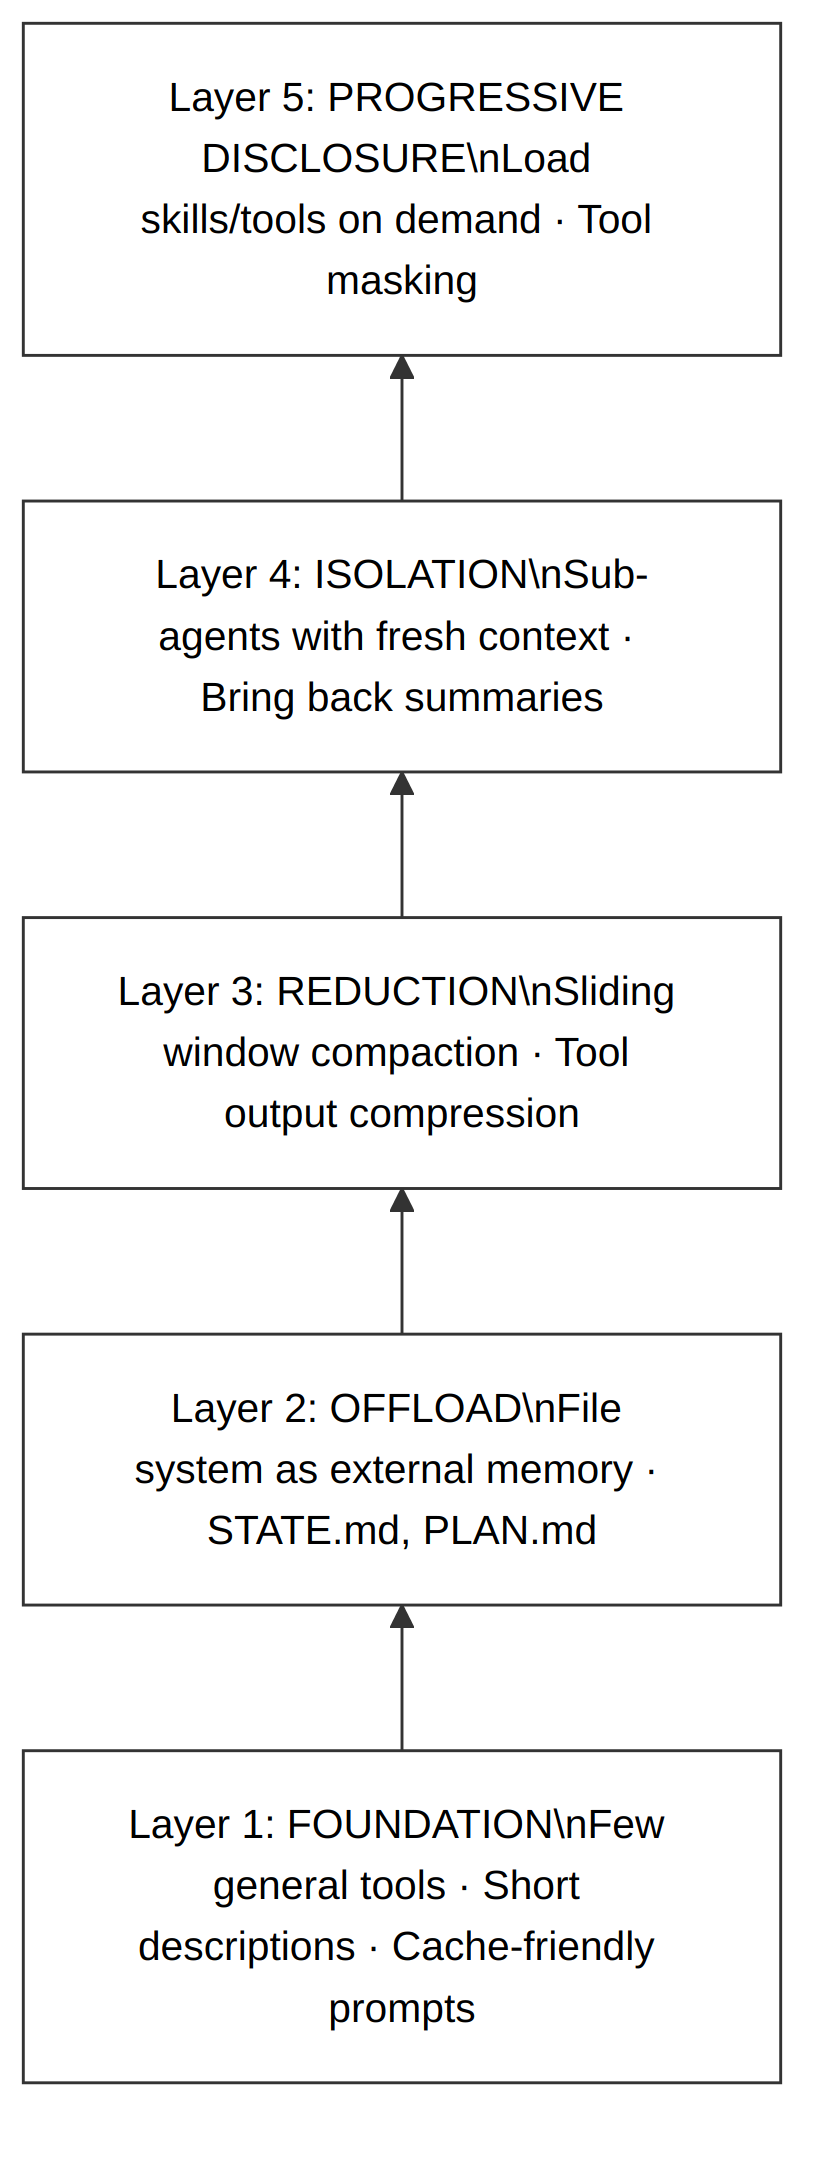
\includegraphics[width=0.85\textwidth,height=\textheight]{figures/diagram_7.png}
\caption{Figure 7. The context engineering stack. Green layers (1--2)
are foundational and should be implemented first. Amber layers (3--4)
address growth and complexity. The blue layer (5) is an optimization
that compounds on a solid foundation}
\end{figure}

Start at Layer 1: design your tools well, keep descriptions short, and
structure your prompts for cache efficiency. Then implement Layer 2:
write state to files instead of keeping it in conversation. Only after
these foundations are solid should you implement compaction (Layer 3),
sub-agent isolation (Layer 4), or progressive disclosure (Layer 5).
Attempting Layer 4 without Layer 2 --- spawning sub-agents that have no
file-based state to share --- creates coordination problems that negate
the benefits of isolation.

\begin{center}\rule{0.5\linewidth}{0.5pt}\end{center}

\hypertarget{multi-agent-systems-coordination-and-frameworks}{%
\subsection{5. Multi-Agent Systems: Coordination and
Frameworks}\label{multi-agent-systems-coordination-and-frameworks}}

\hypertarget{when-multiple-agents-are-necessary}{%
\subsubsection{5.1 When Multiple Agents Are
Necessary}\label{when-multiple-agents-are-necessary}}

The short answer is: almost never. Research by VentureBeat found that
single-agent systems outperform multi-agent systems by a factor of two
to six on tasks involving ten or more tools (VentureBeat, 2025). Context
fragmentation across multiple agents --- each with partial information
about the overall task --- typically exceeds any coordination benefits.
Google's internal research found that multi-agent systems experienced
performance drops of thirty-nine to seventy percent compared to
single-agent baselines, while simultaneously multiplying token costs
(Google Research, 2025).

Multi-agent systems are appropriate in a narrow set of circumstances:

\textbf{Genuine parallelism.} When a task decomposes into truly
independent sub-tasks with no dependencies, running them in parallel
through separate agents can reduce wall-clock time significantly. A
literature review that needs to search five independent databases can
assign each search to a separate agent. But note: this is
parallelization (Pattern 4 from Section 3.1), which does not require a
framework --- it can be implemented with Python's
\passthrough{\lstinline!asyncio!} and a list of tasks.

\textbf{Fundamentally different system prompts.} When sub-tasks require
such different instructions that a single system prompt cannot serve
both well. A code review agent needs different instructions than a code
generation agent. A medical triage agent needs different context than a
billing inquiry agent.

\textbf{Adversarial dynamics.} When the quality of output improves
through critique. A generator agent produces a draft; a reviewer agent
critiques it; the generator revises based on the critique. This pattern
is well-supported by research --- the Reflexion architecture
demonstrated an eighteen-percent accuracy improvement through
self-critique (Shinn et al., 2023) --- but it doubles the token cost.

\textbf{Context window limitations.} When the total information needed
for a task genuinely exceeds a single context window. This is
increasingly rare as context windows grow (Claude Opus 4.6 supports up
to one million tokens in beta), but remains relevant for tasks involving
very large codebases or document corpora.

If none of these conditions apply --- and for most tasks, they do not
--- use a single agent with well-designed tools. The coordination
overhead of multi-agent systems is not zero, and the compounding
reliability problem (Section 2.3) applies to inter-agent communication
just as it applies to individual tool calls.

\hypertarget{communication-patterns}{%
\subsubsection{5.2 Communication
Patterns}\label{communication-patterns}}

When multiple agents are necessary, they must communicate. Four patterns
exist, each with distinct trade-offs.

\begin{figure}
\centering
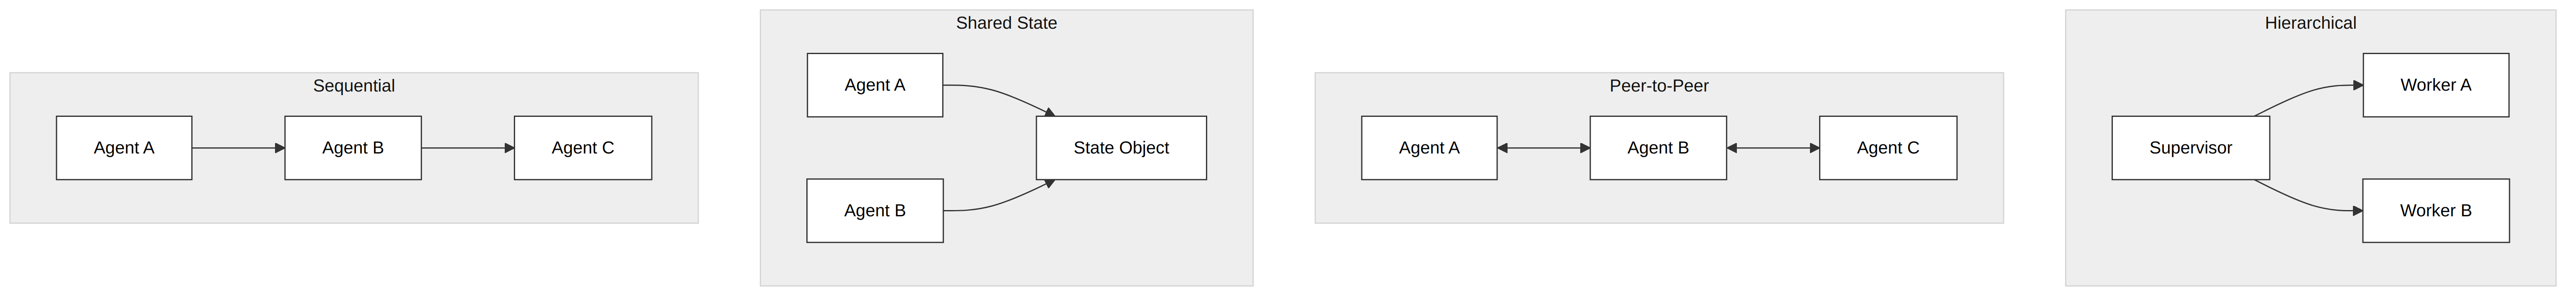
\includegraphics[width=0.85\textwidth,height=\textheight]{figures/diagram_8.png}
\caption{Figure 8. The four multi-agent communication patterns.
Hierarchical delegation is the most predictable. Peer-to-peer is the
most flexible but risks circular conversations. Shared state provides
explicit coordination. Sequential handoff is the simplest but offers no
parallelism}
\end{figure}

\textbf{Hierarchical delegation} is the most predictable pattern. A
supervisor agent examines the task, decomposes it, delegates sub-tasks
to specialized workers, and synthesizes their results. Workers never
communicate with each other --- all coordination flows through the
supervisor. CrewAI (in hierarchical mode), the Claude Agent SDK, and
LangGraph's supervisor pattern all implement this model. Its strength is
predictability: the supervisor is a single decision-maker, and the
communication graph is a star topology that is easy to reason about and
debug.

\textbf{Peer-to-peer communication} (group chat) allows agents to
message each other directly. AutoGen implements this through
\passthrough{\lstinline!RoundRobinGroupChat!} and
\passthrough{\lstinline!SelectorGroupChat!}, where either a turn-based
protocol or an LLM selector determines which agent speaks next. This
pattern is flexible --- agents can build on each other's contributions
--- but carries a significant risk: conversations can spiral without
converging, consuming tokens as agents repeatedly rephrase or contradict
each other. Strong termination conditions are essential.

\textbf{Shared state} gives all agents read-write access to a common
data structure. LangGraph's \passthrough{\lstinline!StateGraph!} is the
clearest implementation: every node (agent) reads from and writes to a
typed state dictionary, with reducers controlling how concurrent updates
are merged. This provides explicit coordination without message-passing
overhead, but requires careful state design to avoid conflicts.

\textbf{Sequential handoff} passes the conversation from one agent to
the next, like a relay baton. OpenAI's Swarm framework (now superseded
by the OpenAI Agents SDK) implements this with approximately 500 lines
of code. Only one agent is active at a time. It is the simplest
multi-agent pattern and is well-suited to routing workflows --- a triage
agent determines the customer's need and hands off to the appropriate
specialist --- but offers no parallelism.

\hypertarget{framework-landscape}{%
\subsubsection{5.3 Framework Landscape}\label{framework-landscape}}

Six frameworks currently dominate the multi-agent space. Rather than
exhaustive documentation (which is available in the companion research
file
\passthrough{\lstinline!research/agents\_framework\_comparison.md!}),
this section provides the essential character of each and guidance on
selection.

\textbf{LangGraph} (LangChain) models agents as directed graphs with
typed state. Its distinguishing feature is \textbf{checkpointing}: every
node execution is automatically persisted, enabling pause-and-resume,
time-travel debugging, and fault-tolerant execution. LangGraph is the
most mature option for complex, stateful workflows with
human-in-the-loop requirements. Its weakness is a steep learning curve
--- the graph programming model (nodes, edges, reducers, conditional
routing) is unfamiliar to most developers. A detailed treatment of
LangGraph's architecture is provided in Appendix A and in
\passthrough{\lstinline!research/agents\_langgraph\_deep\_dive.md!}.

\textbf{CrewAI} uses a role-based mental model: you define agents with
roles (``Senior Research Analyst''), goals, and backstories, then
organize them into crews that execute tasks sequentially or
hierarchically. It is the most intuitive framework for non-technical
stakeholders and the fastest path to a working prototype. Its weakness
is token overhead --- each agent's role and backstory are included in
every LLM call, adding approximately thirty percent to token costs.

\textbf{AutoGen} (Microsoft) models multi-agent coordination as group
chat. Its strength is flexibility: round-robin turns, LLM-selected
speakers, graph-based flows, and built-in code execution. Its weakness
is API instability --- the transition from v0.2 to v0.4 was a breaking
rewrite, and Microsoft is now merging AutoGen with Semantic Kernel into
the Microsoft Agent Framework (targeting 1.0 GA in Q1 2026).

\textbf{smolagents} (Hugging Face) takes a radical stance: agents should
generate Python code rather than JSON tool calls. The LLM writes
\passthrough{\lstinline!result = search("query")!} as executable Python,
which is run in a sandbox. This reduces LLM calls by approximately
thirty percent on complex benchmarks because code naturally supports
composition, control flow, and variable reuse. Its strength is
simplicity and model-agnosticism. Its weakness is that code execution is
an inherent security surface.

\textbf{Claude Agent SDK} (Anthropic) is fundamentally different from
the other frameworks. Instead of providing abstractions for
orchestrating LLM calls, it gives you Claude Code as a library --- an
agent with built-in tools (file reading, code editing, bash execution,
web search) that operates autonomously on a codebase. You do not
implement tool execution; the tools are already implemented and
production-tested. Its strength is zero setup cost for codebase-oriented
tasks. Its weakness is complete vendor lock-in to Anthropic's models.

\textbf{Swarm} (OpenAI) is approximately 500 lines of code wrapping the
Chat Completions API. It is stateless, supports only sequential
handoffs, and is explicitly experimental. OpenAI has released the OpenAI
Agents SDK as its production successor. Swarm remains valuable as a
learning tool --- you can read the entire source code in twenty minutes
and understand what multi-agent coordination actually means at a
mechanical level.

\hypertarget{choosing-a-framework}{%
\subsubsection{5.4 Choosing a Framework}\label{choosing-a-framework}}

\begin{figure}
\centering
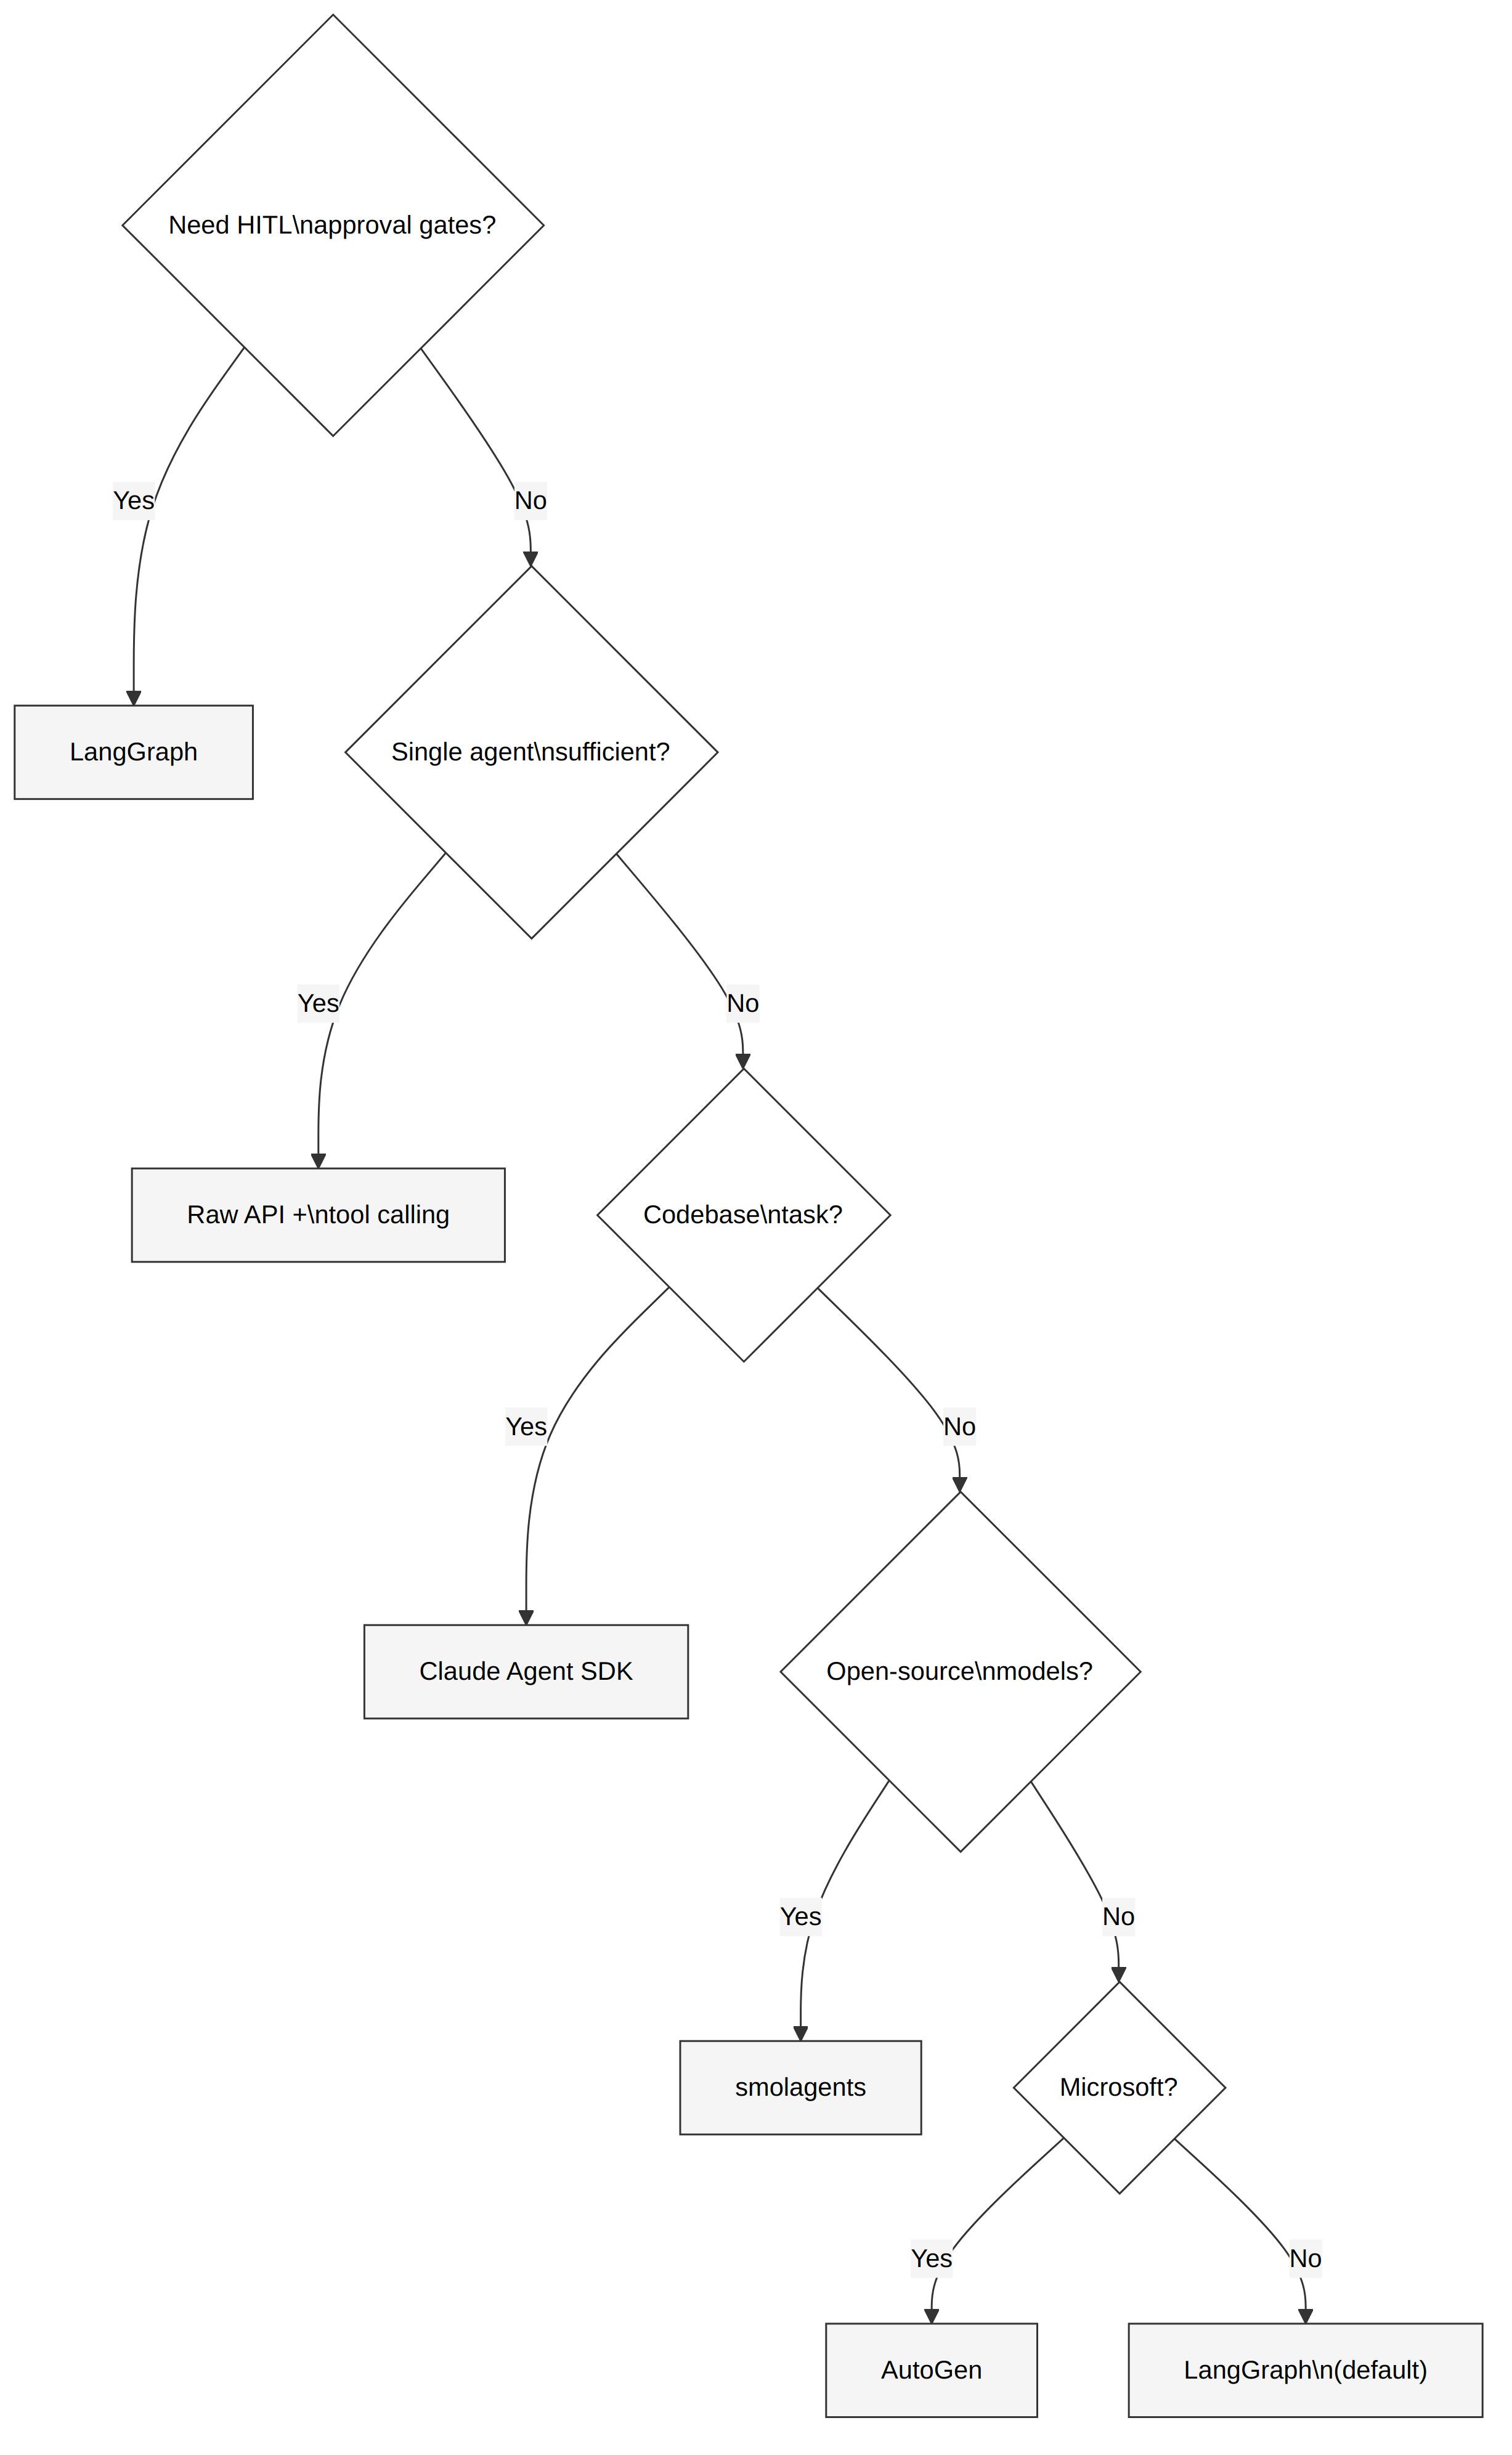
\includegraphics[width=0.85\textwidth,height=\textheight]{figures/diagram_9.png}
\caption{Figure 9. Framework decision tree. Start from the top and
follow the path that matches your requirements. The most common answer
--- ``single agent sufficient'' --- leads to the simplest option}
\end{figure}

\hypertarget{the-cost-of-multi-agent-systems}{%
\subsubsection{5.5 The Cost of Multi-Agent
Systems}\label{the-cost-of-multi-agent-systems}}

Multi-agent systems multiply costs in ways that are not immediately
obvious. Each additional agent adds its own system prompt to every API
call. The supervisor agent pays for its system prompt plus the
conversation history, which includes the outputs of every worker.
Workers generate outputs that become part of the supervisor's context,
and the supervisor's instructions become part of the workers' context in
hierarchical setups.

Concrete numbers: a four-agent CrewAI crew running a
research-and-writing pipeline costs approximately \$0.15 to \$0.50 per
run with GPT-4o. In hierarchical mode, the manager agent roughly doubles
this. An AutoGen group chat with three agents and loose termination
conditions can reach \$0.50 to \$2.00 for complex debates. The Claude
Agent SDK, using Claude Sonnet for sub-agents that read files and run
searches, costs \$0.10 to \$0.50 per task; complex tasks with Claude
Opus can reach \$3.00.

These costs compound with usage. An organization running a multi-agent
pipeline a hundred times per day at \$0.50 per run pays \$15,000 per
year --- for a single workflow. Token prices have dropped dramatically
(280-fold over two years, per Deloitte), but total enterprise AI
spending is increasing because cheaper tokens incentivize more complex
architectures that consume exponentially more tokens. This is Jevons
Paradox\footnote{\textbf{Jevons Paradox} is the observation from
  economics that technological improvements in resource efficiency tend
  to increase, rather than decrease, total resource consumption. As
  coal-burning engines became more efficient in the 19th century, total
  coal consumption rose because the engines became economically viable
  for more applications. The same dynamic applies to AI tokens: cheaper
  tokens enable more complex agent architectures that consume more total
  tokens.} applied to AI: efficiency improvements increase total
consumption.

\begin{center}\rule{0.5\linewidth}{0.5pt}\end{center}

\hypertarget{evaluation-and-observability-knowing-whether-it-works}{%
\subsection{6. Evaluation and Observability: Knowing Whether It
Works}\label{evaluation-and-observability-knowing-whether-it-works}}

\hypertarget{why-agent-evaluation-is-different}{%
\subsubsection{6.1 Why Agent Evaluation Is
Different}\label{why-agent-evaluation-is-different}}

Traditional software testing operates on deterministic systems. Given
input X, the system produces output Y. If Y matches the expected value,
the test passes. If it does not, the test fails. This paradigm breaks
down for agents in three fundamental ways.

\textbf{Non-determinism.} The same prompt with identical context can
produce different tool call sequences, different intermediate reasoning,
and different final outputs across runs. Temperature settings, model
version updates, and even the order of items in the context window
introduce variance. An assertion like
\passthrough{\lstinline!assert output == expected!} is meaningless when
the output varies between runs.

\textbf{Multi-step compounding.} A wrong tool selection in step two does
not merely produce a wrong step-two result --- it poisons every
subsequent step, because later steps operate on a corrupted foundation.
Evaluating only the final output misses the root cause. A correct final
answer produced by an unreliable trajectory is a time bomb: it works
today, but the same fragile path will produce a wrong answer tomorrow on
a slightly different input.

\textbf{Partial success.} An agent that retrieves four of five relevant
documents, calls the right API but with a slightly wrong parameter, or
produces a mostly-correct analysis with one factual error --- is that a
pass or a fail? Binary pass/fail assertions cannot capture the gradient
of quality that characterizes agent outputs. Agent evaluation requires
graded scoring across multiple dimensions.

These challenges mean that agent evaluation must borrow techniques from
domains that have long dealt with non-deterministic, multi-step
processes --- domains like medical trial evaluation, educational
assessment, and qualitative research. The toolbox is unfamiliar to most
software engineers, which is why this chapter exists.

\hypertarget{the-three-evaluation-granularities}{%
\subsubsection{6.2 The Three Evaluation
Granularities}\label{the-three-evaluation-granularities}}

Agent evaluation operates at three levels of granularity, each
corresponding to one level of the Run-Trace-Thread hierarchy\footnote{A
  \textbf{run} is a single LLM call with its input and output. A
  \textbf{trace} links multiple runs into a complete task execution. A
  \textbf{thread} groups multiple traces into a multi-turn session.
  Together they form a hierarchy: Thread → Trace → Run.}.

\textbf{Run-level evaluation (single-step).} Isolate one decision point
and verify it. Given a specific state --- the conversation history, the
available tools, the current context --- did the agent select the
correct tool with the correct arguments? This is the closest analog to
unit testing. It is deterministic (the same frozen state should produce
the same tool call), fast to execute, and pinpoints failures precisely.

For our research agent, a run-level test might verify: given a state
where the agent has searched for papers and found three results, does it
choose to read the most relevant one (based on title match to the query)
rather than reading all three sequentially?

\textbf{Trace-level evaluation (trajectory).} Evaluate the full
execution path of a single task. Did the agent take a reasonable
sequence of steps? Were those steps efficient (minimal unnecessary
actions)? Did the final output satisfy the task requirements?

Two approaches exist for trace evaluation. \textbf{Trajectory matching}
compares the agent's actual tool call sequence against a reference
trajectory, with configurable strictness --- exact order match,
unordered match (same tools, any order), or subset match (reference
tools must appear, extras allowed). \textbf{LLM-as-judge} uses a
separate model to evaluate whether the trajectory was reasonable,
scoring dimensions like tool selection quality, efficiency, and
completeness.

LLM-as-judge evaluations require careful design. Research shows that
naive implementations exhibit position bias (preferring the first option
presented), length bias (preferring longer responses), and agreeableness
bias (reluctant to give low scores), with error rates exceeding fifty
percent in some configurations (Evidently AI, 2025). Mitigations include
explicit rubrics with scoring examples, requiring the judge to provide
evidence before scoring, running multiple evaluations with randomized
presentation order, and calibrating against human expert judgments.

\textbf{Thread-level evaluation (conversation).} The most difficult
level. Does the agent maintain context across multiple user turns? Does
it remember preferences stated in turn one when responding in turn five?
Does it handle corrections gracefully? Thread-level evaluation is
essential for conversational agents and agents with persistent memory
systems, but it requires test scripts that simulate multi-turn
interactions and scoring criteria that capture coherence over time.

\hypertarget{the-evaluation-lifecycle}{%
\subsubsection{6.3 The Evaluation
Lifecycle}\label{the-evaluation-lifecycle}}

Effective agent evaluation involves three complementary modes that
operate at different points in the development lifecycle.

\textbf{Offline evaluation} runs before deployment, typically as part of
a continuous integration pipeline. The agent is tested against a curated
dataset of inputs with known-good outputs or reference trajectories.
This catches regressions before they reach production. According to the
LangChain State of Agent Engineering survey (1,340 respondents, December
2025), 52.4\% of organizations run offline evaluations on test sets.

\textbf{Online evaluation} runs during production. It scores a sample of
live traces using reference-free evaluators --- no expected output is
needed because the evaluator assesses quality from the trace alone.
Online evaluation detects quality degradation, cost anomalies, and
behavioral drift that offline tests cannot anticipate. The same survey
found that 89\% of organizations have implemented some form of
production observability.

\textbf{Ad-hoc evaluation} is the investigative mode. When a user
reports a problem or an anomaly alert fires, a developer examines
specific traces to diagnose the issue. The most valuable outcome of
ad-hoc evaluation is the \textbf{trace-to-test-case conversion}: every
diagnosed failure becomes a new entry in the offline test dataset,
preventing the same failure from recurring.

These three modes form a flywheel: online monitoring detects problems,
ad-hoc investigation diagnoses them, and the resulting test cases
strengthen offline evaluation, which prevents recurrence. Organizations
that implement all three modes --- and close the loop between them ---
see continuous improvement in agent reliability.

\hypertarget{practical-evaluation-patterns}{%
\subsubsection{6.4 Practical Evaluation
Patterns}\label{practical-evaluation-patterns}}

Four concrete patterns cover the majority of agent evaluation needs.
Each is presented with enough detail to implement.

\textbf{Pattern 1: Assertion-based tool call verification.}
Deterministic checks on the agent's behavior, requiring no LLM judge.
Verify that a specific tool was called, that a dangerous tool was
\emph{not} called, that tools were called in the expected order, or that
a tool was called with specific arguments. These tests are fast, cheap,
and highly reliable --- they should form the foundation of any
evaluation suite.

\textbf{Pattern 2: LLM-as-judge for trajectory quality.} A judge model
evaluates the agent's execution path against explicit criteria: was the
tool selection appropriate? Was the path efficient? Were the arguments
correct? Was all necessary information gathered? Was the final output
complete? The judge returns numerical scores (typically 1--5 per
criterion) and a textual explanation. The explanation serves both as a
debugging aid and as a check on the judge's own reasoning.

\textbf{Pattern 3: Reference-based output comparison.} For tasks with
verifiable answers, compare the agent's output against a known-good
reference. A judge model determines whether the agent's answer contains
all the facts in the reference, identifies missing facts and incorrect
facts, and returns a score from 0.0 (completely wrong) to 1.0 (all facts
present and correct). This pattern is appropriate for factual research
tasks, data extraction, and structured analysis.

\textbf{Pattern 4: Cost and latency tracking.} Non-negotiable for
production agents. Track total tokens, total cost, total latency, number
of LLM calls, and number of tool calls per trace. Set anomaly thresholds
at three times the historical median --- a trace that costs three times
the median cost likely indicates a loop, an error cascade, or a
dramatically unusual input. These metrics are cheap to compute (no LLM
judge required) and provide the earliest warning of operational
problems.

Implementation code for all four patterns is provided in
\passthrough{\lstinline!scripts/agents/eval\_harness.py!}.

\hypertarget{the-evaluation-tool-landscape}{%
\subsubsection{6.5 The Evaluation Tool
Landscape}\label{the-evaluation-tool-landscape}}

Several platforms provide infrastructure for agent evaluation and
observability. The choice depends primarily on your existing stack:

\textbf{LangSmith} (by LangChain) provides native integration with
LangChain and LangGraph, offering trace visualization, annotation queues
for human review, and pairwise comparison between agent versions. Best
for teams already in the LangChain ecosystem. Per-seat pricing.

\textbf{Braintrust} focuses on evaluation-driven deployment governance.
Its distinguishing feature is one-click conversion from a production
trace to an offline test case, closing the evaluation flywheel with
minimal friction. Native GitHub Actions integration blocks code merges
when quality metrics regress. Framework-agnostic with 40+ integrations.
Usage-based pricing.

\textbf{Phoenix} (by Arize) is open source and built on OpenTelemetry
standards. It accepts traces in the standard OTLP wire format, meaning
you can instrument your agent once and send traces to any
OTLP-compatible backend. Best for teams that want vendor independence
and self-hosted infrastructure.

\textbf{Langfuse} is open source and self-hostable, providing tracing,
scoring, and dataset management. Its
\passthrough{\lstinline!instrument\_all()!} function provides
auto-instrumentation for supported frameworks with a single function
call. Good for teams that want full control over their evaluation
infrastructure.

The practical recommendation: start with whichever platform requires the
least integration effort for your current stack. The choice of
evaluation platform matters far less than the choice to evaluate at all.

\begin{center}\rule{0.5\linewidth}{0.5pt}\end{center}

\hypertarget{production-safety-cost-and-human-oversight}{%
\subsection{7. Production: Safety, Cost, and Human
Oversight}\label{production-safety-cost-and-human-oversight}}

\hypertarget{the-failure-rate-reality}{%
\subsubsection{7.1 The Failure Rate
Reality}\label{the-failure-rate-reality}}

The gap between agent demonstrations and production deployments is the
largest credibility problem in current AI. The following table
summarizes the empirical evidence as of early 2026:

\emph{Table 1. Agent failure rates and deployment statistics from major
studies and surveys.}

\begin{longtable}[]{@{}
  >{\raggedright\arraybackslash}p{(\columnwidth - 4\tabcolsep) * \real{0.3750}}
  >{\raggedright\arraybackslash}p{(\columnwidth - 4\tabcolsep) * \real{0.2917}}
  >{\raggedright\arraybackslash}p{(\columnwidth - 4\tabcolsep) * \real{0.3333}}@{}}
\toprule\noalign{}
\begin{minipage}[b]{\linewidth}\raggedright
Finding
\end{minipage} & \begin{minipage}[b]{\linewidth}\raggedright
Value
\end{minipage} & \begin{minipage}[b]{\linewidth}\raggedright
Source
\end{minipage} \\
\midrule\noalign{}
\endhead
\bottomrule\noalign{}
\endlastfoot
Enterprise AI pilots failing to reach production & 95\% & MIT/Fortune
(Zhang, 2025) \\
Agentic AI tasks failing on real CRM workflows & 75\% & Superface
(2025) \\
Agentic AI projects predicted to be scrapped by 2027 & 40\% & Gartner
(2025) \\
Multi-agent pilots failing within 6 months & 40\% & Gartner (2025) \\
Organizations with agentic AI in production & 11\% & Cleanlab (2025) \\
Developers actually slower when using AI tools & 19\% & METR (2025) \\
\end{longtable}

These numbers are not evidence that agents are useless. They are
evidence that the deployment approach is immature. The organizations
succeeding with agents share five characteristics: they choose bounded
problems, build human-in-the-loop from day one, measure actual outcomes
(not perceptions), start with single agents before attempting
multi-agent, and apply the two-way door principle for agent autonomy.

\hypertarget{non-negotiable-safety-controls}{%
\subsubsection{7.2 Non-Negotiable Safety
Controls}\label{non-negotiable-safety-controls}}

Every production agent system requires the following controls. These are
not optional enhancements --- they are the minimum baseline for
responsible deployment.

\emph{Table 2. Required safety controls for production agent systems.}

\begin{longtable}[]{@{}
  >{\raggedright\arraybackslash}p{(\columnwidth - 4\tabcolsep) * \real{0.2045}}
  >{\raggedright\arraybackslash}p{(\columnwidth - 4\tabcolsep) * \real{0.2955}}
  >{\raggedright\arraybackslash}p{(\columnwidth - 4\tabcolsep) * \real{0.5000}}@{}}
\toprule\noalign{}
\begin{minipage}[b]{\linewidth}\raggedright
Control
\end{minipage} & \begin{minipage}[b]{\linewidth}\raggedright
What It Does
\end{minipage} & \begin{minipage}[b]{\linewidth}\raggedright
Implementation Effort
\end{minipage} \\
\midrule\noalign{}
\endhead
\bottomrule\noalign{}
\endlastfoot
\textbf{Iteration cap} & Stops the agent after N tool calls & 5 lines of
code \\
\textbf{Token budget} & Maximum tokens per task, per hour, per day &
Configuration \\
\textbf{Time limit} & Maximum execution duration before termination &
Configuration \\
\textbf{Cost cap} & Maximum dollar spend per task and per day &
Monitoring integration \\
\textbf{Circuit breaker} & Halts execution on anomalous behavior
patterns & Medium \\
\textbf{Kill switch} & Human-accessible emergency stop for any agent &
Low \\
\textbf{Audit log} & Immutable record of every action taken & Medium \\
\end{longtable}

The \$47,000 runaway agent incident --- where two agents in a research
loop ran for eleven days without supervision --- could have been
prevented by any single control in this table. The agent had no
iteration cap, no cost limit, no time limit, and no monitoring. Every
production deployment must have all seven.

\hypertarget{human-in-the-loop-design}{%
\subsubsection{7.3 Human-in-the-Loop
Design}\label{human-in-the-loop-design}}

Human oversight is not a concession to immaturity. It is the
architecture that makes agents production-viable. The most effective
deployment pattern is \textbf{bounded autonomy}: the agent operates
freely within defined boundaries, and stops to ask when it approaches or
reaches those boundaries.

\textbf{The two-way door principle in practice.} Classify every action
the agent can take as either reversible or irreversible:

\begin{itemize}
\tightlist
\item
  \textbf{Reversible actions} (creating a draft, generating a code
  suggestion, querying a database, writing to a scratch file): allow the
  agent to act autonomously. Speed matters more than caution.
\item
  \textbf{Irreversible actions} (sending a message to a client,
  deploying to production, spending money, deleting data, modifying a
  production database): require explicit human approval before
  execution.
\end{itemize}

The boundary between these categories is domain-specific. In a medical
context, generating a triage recommendation is reversible (a human
reviews it before acting), but sending a prescription is irreversible.
In a financial context, drafting a trade is reversible, but executing it
is irreversible. Map these boundaries explicitly for your domain before
building the agent.

\textbf{Confidence-based escalation.} The agent can provide a confidence
score alongside its decisions. When confidence exceeds a
domain-appropriate threshold (typically eighty to ninety-five percent,
depending on the stakes), the decision proceeds automatically. Below the
threshold, the decision routes to a human reviewer. The operational
target for escalation rate is ten to fifteen percent --- low enough that
the agent provides genuine value, but high enough that edge cases
receive human attention. Above fifteen percent escalation, you have
built an expensive ticketing system, not an agent.

\hypertarget{state-management-across-sessions}{%
\subsubsection{7.4 State Management Across
Sessions}\label{state-management-across-sessions}}

Agents that operate across multiple sessions --- which includes most
production agents --- need persistent state that survives context window
resets, session boundaries, and process restarts.

The effective stack, informed by the context engineering principles from
Chapter 4, consists of three layers:

\textbf{Layer 1: STATE.md.} A markdown file tracking the agent's current
phase, progress, key decisions, and blockers. Written at session end,
loaded at session start. Serves as the agent's ``short-term memory'' ---
what was I doing, and what comes next?

\textbf{Layer 2: Episodic log.} An append-only log where each session's
key observations are distilled into three to five lines and appended to
a JSONL file. Serves as the agent's ``long-term memory'' --- what has
happened over time? The most recent five to ten entries are loaded at
session start to provide continuity.

\textbf{Layer 3: File system.} The ground truth for all persistent
artifacts --- research findings, generated code, configuration, plans.
Files are version-controlled through git, providing complete history and
rollback capability.

Ronacher's formulation captures the philosophy: ``Agent memory isn't
model learning. It's state ownership + rehydration'' (Ronacher, 2026).
The model does not ``remember'' anything between sessions. It reads
files, operates on them, writes updates, and terminates. The next
session begins by reading the same files. Continuity is a property of
the file system, not of the model.

\hypertarget{cost-monitoring-and-control}{%
\subsubsection{7.5 Cost Monitoring and
Control}\label{cost-monitoring-and-control}}

Track costs at three levels of granularity:

\textbf{Per-trace} (individual task): total tokens multiplied by
model-specific pricing. Alert when a single trace exceeds three times
the historical median cost --- this indicates a possible loop, error
cascade, or unusually complex input.

\textbf{Per-day} (aggregate): total spending across all agent
invocations. Set a hard daily cap that cannot be exceeded without manual
override. The cap should be set with reference to the value the agent
provides --- if the agent saves two hours of human time per day, and
human time costs \$50 per hour, the agent's daily cost should not exceed
\$100.

\textbf{Per-task-type} (analytical): which categories of tasks are most
expensive? This analysis often reveals that a small number of task types
account for the majority of spending. Optimizing those specific
workflows --- through better context management, more efficient tool
designs, or caching of repeated queries --- yields disproportionate
savings.

\begin{center}\rule{0.5\linewidth}{0.5pt}\end{center}

\hypertarget{implementation-building-it-step-by-step}{%
\subsection{8. Implementation: Building It Step by
Step}\label{implementation-building-it-step-by-step}}

This chapter connects the concepts from earlier chapters to runnable
code. All implementations are available in
\passthrough{\lstinline!scripts/agents/!} and are designed to be
readable as educational material --- someone studying the code should
learn how agents work, not just how to call an API.

\hypertarget{the-react-agent}{%
\subsubsection{8.1 The ReAct Agent}\label{the-react-agent}}

\passthrough{\lstinline!scripts/agents/react\_agent.py!} implements a
complete ReAct agent with: - A think-act-observe loop using the
OpenAI-compatible API (works with Groq, local models, and other
providers) - A circuit breaker with configurable maximum iterations
(default: 10) - Structured tool calling via function calling (not
free-text parsing) - Full audit trail logging every thought, action, and
observation - Per-run cost tracking based on token counts and model
pricing

The implementation is approximately 150 lines of Python. The core loop
--- the think-act-observe cycle --- is fifteen lines. The remaining code
handles tool registration, error wrapping, cost tracking, and the audit
trail. This ratio --- fifteen lines of core logic and 135 lines of
scaffolding --- is itself an illustration of the Scaffolding
\textgreater{} Models principle from Section 3.6.

\hypertarget{the-tool-registry}{%
\subsubsection{8.2 The Tool Registry}\label{the-tool-registry}}

\passthrough{\lstinline!scripts/agents/tool\_definitions.py!} provides a
reusable tool registry pattern: - A \passthrough{\lstinline!@tool!}
decorator that converts a Python function into an agent-callable tool,
automatically generating the JSON Schema from type hints and docstrings
- A \passthrough{\lstinline!ToolRegistry!} that manages tool lookup,
validation, and schema generation - Error wrapping that converts tool
failures into actionable messages (telling the model what to do
differently, not just showing a stack trace) - Export in both OpenAI and
Anthropic schema formats

\hypertarget{file-based-state-management}{%
\subsubsection{8.3 File-Based State
Management}\label{file-based-state-management}}

\passthrough{\lstinline!scripts/agents/state\_manager.py!} implements
the three-layer state management approach from Section 7.4: -
\passthrough{\lstinline!PlanManager!} --- maintains a PLAN.md file with
checkboxes for each step - \passthrough{\lstinline!StateManager!} ---
maintains a STATE.md file with key-value metadata -
\passthrough{\lstinline!EpisodicLog!} --- appends timestamped
observations to a JSONL file - \passthrough{\lstinline!AgentWorkspace!}
--- combines all three into a directory-based workspace

\hypertarget{the-evaluation-harness}{%
\subsubsection{8.4 The Evaluation
Harness}\label{the-evaluation-harness}}

\passthrough{\lstinline!scripts/agents/eval\_harness.py!} implements the
four evaluation patterns from Section 6.4: - Test case definition with
expected outputs, required tool calls, and forbidden tool calls -
Configurable validators (exact match, contains, number comparison,
any-of) - Built-in test suites for verification (math, reasoning) - Cost
and latency tracking per test case - Markdown and JSON report generation

\hypertarget{the-supervisor-agent}{%
\subsubsection{8.5 The Supervisor Agent}\label{the-supervisor-agent}}

\passthrough{\lstinline!scripts/agents/supervisor\_agent.py!} implements
the hierarchical multi-agent pattern from Section 5.2: - A supervisor
that decomposes tasks and delegates to specialized workers -
Pre-configured worker profiles (researcher, writer, critic, analyst) -
Star topology --- workers never communicate directly - Optional
human-in-the-loop approval gate for critical decisions - Aggregate cost
tracking across all agents

\hypertarget{adding-memory}{%
\subsubsection{8.6 Adding Memory}\label{adding-memory}}

For agents that operate across sessions, the
\passthrough{\lstinline!EpisodicLog!} from Section 8.3 provides the
foundation. At the end of each session, the agent distills its key
observations into three to five lines and appends them to the log. At
the start of the next session, the most recent entries are loaded into
context, providing continuity without consuming excessive tokens.

For semantic retrieval over accumulated knowledge --- finding relevant
past observations based on meaning rather than recency --- combine the
episodic log with a vector database. The pattern:

\begin{enumerate}
\def\labelenumi{\arabic{enumi}.}
\tightlist
\item
  \textbf{At session end:} Distill observations. Embed each observation
  using a text embedding model. Store embeddings in the vector database
  alongside the observation text and metadata (timestamp, session ID,
  tags).
\item
  \textbf{At session start:} Query the vector database with the current
  task description. Retrieve the top five most relevant past
  observations. Inject them into the agent's context.
\item
  \textbf{Temporal decay:} Weight recent observations higher than older
  ones. An observation from yesterday is more likely to be relevant than
  one from three months ago.
\end{enumerate}

This is the minimum viable memory system. More sophisticated approaches
--- knowledge graphs, entity extraction, temporal reasoning --- exist
(Mem0, LightRAG, Graphiti), but as of March 2026, all of them have weak
evidence bases consisting primarily of their own papers and small
benchmarks. The simple version --- episodic log, vector search, temporal
decay --- covers the vast majority of practical memory needs.

\begin{center}\rule{0.5\linewidth}{0.5pt}\end{center}

\hypertarget{conclusion}{%
\subsection{9. Conclusion}\label{conclusion}}

\hypertarget{what-this-manual-has-argued}{%
\subsubsection{What This Manual Has
Argued}\label{what-this-manual-has-argued}}

The central argument of this manual is that building effective AI agents
is primarily an engineering challenge, not a modeling challenge. The
model provides the reasoning capability, but the scaffolding --- the
tool definitions, the context management, the evaluation infrastructure,
the safety controls, the human oversight patterns --- determines whether
that capability translates into reliable, cost-effective production
systems.

The compounding reliability problem (0.95\^{}n) is the fundamental
constraint. Until per-step reliability exceeds ninety-nine percent ---
which no current architecture achieves --- long autonomous chains will
remain mathematically impractical without human checkpoints. The path
forward is not ``wait for better models.'' It is better architecture:
fewer steps, better tools, aggressive context management, thorough
evaluation, and honest acknowledgment of limitations.

\hypertarget{what-works-today}{%
\subsubsection{What Works Today}\label{what-works-today}}

Coding agents with human oversight, customer support deflection, and
structured research assistance are the three categories where agents
deliver genuine value in production. They share common characteristics:
bounded problem spaces, clear success criteria, built-in human review,
and reversible actions. Organizations deploying agents successfully
start with single agents on bounded problems and expand gradually based
on measured results.

\hypertarget{what-does-not-work-yet}{%
\subsubsection{What Does Not Work Yet}\label{what-does-not-work-yet}}

Fully autonomous multi-step business processes, multi-agent coordination
at scale, and general-purpose computer use agents remain aspirational.
The gap between demonstrations and production deployments is the largest
credibility problem in current AI. This gap will narrow as tooling
matures, evaluation practices improve, and the engineering community
accumulates hard-won deployment experience --- but it will not close
overnight.

\hypertarget{limitations-of-this-manual}{%
\subsubsection{Limitations of This
Manual}\label{limitations-of-this-manual}}

This manual reflects the state of the field as of March 2026. The AI
agent landscape changes rapidly: frameworks release breaking updates
quarterly, new architectures emerge monthly, and benchmark results that
were state-of-the-art at writing time may be obsolete within months. The
architectural principles --- context engineering, evaluation, bounded
autonomy, scaffolding over models --- are more durable than the specific
tools and frameworks described here.

The manual draws primarily on English-language sources, open-source
frameworks, and publicly reported deployment data. Enterprise
deployments with proprietary tooling may exhibit different patterns.
Production cost data is aggregated from public reports and the authors'
direct experience; individual deployments will vary based on task
complexity, model choice, and implementation quality.

\hypertarget{what-to-do-next}{%
\subsubsection{What to Do Next}\label{what-to-do-next}}

If you are starting from scratch, implement the automation spectrum
decision (Section 2.2) first. Most tasks do not need agents. For the
tasks that do, build a single ReAct agent (Section 3.2) with a small
number of well-designed tools (Section 3.4), file-based state management
(Section 4.2), and a circuit breaker. Add evaluation (Chapter 6) before
adding capabilities. Add human-in-the-loop (Section 7.3) before
expanding autonomy. Measure everything. Trust measurements over
perceptions.

\begin{center}\rule{0.5\linewidth}{0.5pt}\end{center}

\hypertarget{glossary}{%
\subsection{10. Glossary}\label{glossary}}

\textbf{Agent.} A software system where a large language model
dynamically directs its own processes and tool usage, deciding at
runtime which actions to take based on intermediate results.

\textbf{Circuit breaker.} A mechanism that stops an agent after a
predetermined number of steps, elapsed time, or dollar cost, preventing
runaway execution.

\textbf{Compounding reliability problem.} The mathematical observation
that multi-step agents with less-than-perfect per-step reliability
experience exponentially declining overall success rates (0.95\^{}n for
95\% per-step reliability).

\textbf{Context engineering.} The discipline of managing what
information a language model sees at each step --- including retrieved
documents, conversation history, tool definitions, and state --- to
maximize the model's effectiveness.

\textbf{Context rot.} The degradation of model performance as context
window size increases, due to ``lost in the middle'' effects and
attention dilution.

\textbf{Hallucination.} When a language model generates plausible but
factually incorrect information, including fabricated tool calls,
non-existent API parameters, or false citations.

\textbf{Human-in-the-loop (HITL).} An architecture pattern where human
review and approval are integrated into the agent's execution flow at
predetermined decision points.

\textbf{KV cache.} Key-value cache used by transformer models to avoid
recomputing attention over previously processed tokens. Context changes
that invalidate the cache increase cost and latency.

\textbf{MCP (Model Context Protocol).} A standard for connecting AI
models to external tools, providing a uniform interface for tool
definitions, developed by Anthropic.

\textbf{ReAct.} ``Reason + Act.'' An agent architecture where the model
alternates between reasoning about the current state and taking an
action, creating a loop that continues until the task is complete.

\textbf{Recency bias.} The tendency of transformer models to pay more
attention to tokens near the end of the context window, influencing both
retrieval accuracy and instruction following.

\textbf{Scaffolding.} The non-model components of an agent system: tool
definitions, error handling, context management, evaluation
infrastructure, safety controls, and deployment configuration.

\textbf{Token.} A unit of text processed by a language model. One token
is approximately four characters or three-quarters of a word in English.
Tokens are the billing unit for API-based language models.

\textbf{Trace.} A complete record of an agent's execution for a single
task, including all LLM calls, tool invocations, intermediate reasoning,
and the final output.

\textbf{Two-way door principle.} A decision framework distinguishing
reversible decisions (two-way doors, safe for automation) from
irreversible decisions (one-way doors, requiring human approval).

\textbf{Workflow.} A system where LLMs are orchestrated through
predefined code paths. The developer, not the model, decides the control
flow.

\begin{center}\rule{0.5\linewidth}{0.5pt}\end{center}

\hypertarget{references}{%
\subsection{11. References}\label{references}}

Anthropic. (2024, December 20). Building effective agents. Anthropic.
https://www.anthropic.com/research/building-effective-agents

Anthropic. (2025a). Effective context engineering for AI agents.
Anthropic.
https://www.anthropic.com/engineering/effective-context-engineering-for-ai-agents

Anthropic. (2025b). Effective harnesses for long-running agents.
Anthropic.
https://www.anthropic.com/engineering/effective-harnesses-for-long-running-agents

Cleanlab. (2025). AI agents in production 2025. Cleanlab.
https://cleanlab.ai/ai-agents-in-production-2025/

Evidently AI. (2025). LLM-as-a-judge: Complete guide. Evidently AI.
https://www.evidentlyai.com/llm-guide/llm-as-a-judge

Gartner. (2025). Predicts 2026: AI agents and the future of automation.
Gartner.

Google Research. (2025). Multi-agent performance analysis {[}Internal
report, cited in VentureBeat{]}.

Karpathy, A. (2025, December). 2025 LLM year in review. Bear Blog.
https://karpathy.bearblog.dev/year-in-review-2025/

LangChain Team. (2025). State of agent engineering (Survey of 1,340
respondents, December 2025). LangChain.
https://www.langchain.com/state-of-agent-engineering

Manus. (2025). Context engineering for AI agents: Lessons from building
Manus. Manus.
https://manus.im/blog/Context-Engineering-for-AI-Agents-Lessons-from-Building-Manus

Martin, L. (2025, June 23). Context engineering for agents. Personal
blog. https://rlancemartin.github.io/2025/06/23/context\_engineering/

METR. (2025, July 10). Early 2025 AI-experienced open-source developer
study. METR.
https://metr.org/blog/2025-07-10-early-2025-ai-experienced-os-dev-study/

Miessler, D. (2026). Harness engineering {[}Video transcript{]}.
CraftersLab.

Ronacher, A. (2025, November 21). Agents are hard. Personal blog.
https://lucumr.pocoo.org/2025/11/21/agents-are-hard/

Ronacher, A. (2026, January 31). PI. Personal blog.
https://lucumr.pocoo.org/2026/1/31/pi/

Ronacher, A. (2026, February 13). The final bottleneck. Personal blog.
https://lucumr.pocoo.org/2026/2/13/the-final-bottleneck/

Salesforce. (2025). State of service report (5th ed.). Salesforce
Research.

Shinn, N., Cassano, F., Gopinath, A., Narasimhan, K., \& Yao, S. (2023).
Reflexion: Language agents with verbal reinforcement learning. In
\emph{Advances in Neural Information Processing Systems, 36}.

Superface. (2025). The agent reality gap: Why 75\% of AI agent tasks
fail. Superface. https://superface.ai/blog/agent-reality-gap

SWE-bench. (2026). SWE-bench leaderboard. https://www.swebench.com/

Vercel. (2025). We removed 80\% of our agent's tools. Vercel Blog.
https://vercel.com/blog/we-removed-80-percent-of-our-agents-tools

VentureBeat. (2025). Single-agent vs.~multi-agent performance analysis.
VentureBeat.

Yao, S., Zhao, J., Yu, D., Du, N., Shafran, I., Narasimhan, K., \& Cao,
Y. (2023). ReAct: Synergizing reasoning and acting in language models.
In \emph{International Conference on Learning Representations (ICLR)}.

Zechner, M. (2025, June 2). Prompts are code, .json/.md files are state.
Personal blog.
https://mariozechner.at/posts/2025-06-02-prompts-are-code/

Zechner, M. (2025, August 15). MCP vs CLI: Benchmarking tools for coding
agents. Personal blog.
https://mariozechner.at/posts/2025-08-15-mcp-vs-cli/

Zechner, M. (2025, November 30). What I learned building an opinionated
and minimal coding agent. Personal blog.
https://mariozechner.at/posts/2025-11-30-pi-coding-agent/

Zhang, A. L. (2025). 95\% of GenAI pilots failing, MIT report finds.
\emph{Fortune}.
https://fortune.com/2025/08/18/mit-report-95-percent-generative-ai-pilots-at-companies-failing-cfo/

\begin{center}\rule{0.5\linewidth}{0.5pt}\end{center}

\hypertarget{appendices}{%
\subsection{12. Appendices}\label{appendices}}

\hypertarget{appendix-a-langgraph-architecture-reference}{%
\subsubsection{Appendix A: LangGraph Architecture
Reference}\label{appendix-a-langgraph-architecture-reference}}

A comprehensive treatment of LangGraph's architecture --- including
StateGraph construction, checkpointing, human-in-the-loop interrupt
patterns, multi-agent supervisor patterns, and production streaming ---
is provided in the companion file
\passthrough{\lstinline!research/agents\_langgraph\_deep\_dive.md!}.
That document includes complete, runnable code examples for each
pattern.

\hypertarget{appendix-b-framework-comparison-details}{%
\subsubsection{Appendix B: Framework Comparison
Details}\label{appendix-b-framework-comparison-details}}

Detailed evaluations of all six frameworks discussed in Chapter 5 ---
including architecture analysis, code examples, cost estimates, and
honest assessments of limitations --- are provided in
\passthrough{\lstinline!research/agents\_framework\_comparison.md!}.

\hypertarget{appendix-c-evaluation-and-observability-details}{%
\subsubsection{Appendix C: Evaluation and Observability
Details}\label{appendix-c-evaluation-and-observability-details}}

Extended coverage of evaluation patterns, the observability tool
landscape, and a step-by-step implementation guide are provided in
\passthrough{\lstinline!research/agents\_evaluation\_observability.md!}.

\hypertarget{appendix-d-context-engineering-patterns}{%
\subsubsection{Appendix D: Context Engineering
Patterns}\label{appendix-d-context-engineering-patterns}}

Detailed treatment of all four context management strategies --- with
code examples, production data from Manus and Vercel, and the five-layer
context engineering stack --- is provided in
\passthrough{\lstinline!research/agents\_context\_engineering.md!}.

\hypertarget{appendix-e-runnable-code}{%
\subsubsection{Appendix E: Runnable
Code}\label{appendix-e-runnable-code}}

All implementation code referenced in Chapter 8 is available in
\passthrough{\lstinline!scripts/agents/!}:

\begin{longtable}[]{@{}
  >{\raggedright\arraybackslash}p{(\columnwidth - 4\tabcolsep) * \real{0.2308}}
  >{\raggedright\arraybackslash}p{(\columnwidth - 4\tabcolsep) * \real{0.5000}}
  >{\raggedright\arraybackslash}p{(\columnwidth - 4\tabcolsep) * \real{0.2692}}@{}}
\toprule\noalign{}
\begin{minipage}[b]{\linewidth}\raggedright
File
\end{minipage} & \begin{minipage}[b]{\linewidth}\raggedright
Description
\end{minipage} & \begin{minipage}[b]{\linewidth}\raggedright
Lines
\end{minipage} \\
\midrule\noalign{}
\endhead
\bottomrule\noalign{}
\endlastfoot
\passthrough{\lstinline!react\_agent.py!} & ReAct loop with circuit
breaker and cost tracking & \textasciitilde150 \\
\passthrough{\lstinline!tool\_definitions.py!} & @tool decorator,
registry, schema generation & \textasciitilde130 \\
\passthrough{\lstinline!state\_manager.py!} & PLAN.md, STATE.md,
episodic log management & \textasciitilde160 \\
\passthrough{\lstinline!eval\_harness.py!} & Test cases, validators,
eval reports & \textasciitilde155 \\
\passthrough{\lstinline!supervisor\_agent.py!} & Multi-agent supervisor
with human-in-the-loop & \textasciitilde190 \\
\end{longtable}

\hypertarget{appendix-f-source-documents}{%
\subsubsection{Appendix F: Source
Documents}\label{appendix-f-source-documents}}

Primary source documents referenced in this manual are archived in
\passthrough{\lstinline!research/sources/!} for reproducibility.

\end{document}
